\section{Wave Phenomena}

\subsection{The Nature of Waves}
\label{subsection:nature-of-waves}
Typically, a wave is a disturbance that propagates through a medium. There are several types of waves we will discuss in this course, including mechanical, electromagnetic, transverse, longitudinal and stationary waves.


\begin{definition}{(\textbf{Propagate})}
\textit{To propagate refers to the transmission of a disturbance from one location to another.}
\end{definition}
\begin{definition}{(\textbf{Medium})}
\textit{Medium (or media) refers to the intervening substance(s) through which a disturbance is transmitted.}
\end{definition}

However, despite the different types of waves we know that waves must transfer energy, momentum, and information, but not mass. 
We will now discuss the different types of waves based on their mediums, wave orientation or energy transfer.

\subsubsection{Types of waves classed by media}
\begin{itemize}
    \item \textbf{Mechanical Waves} \\
    Mechanical waves, such as water or sound waves, travel within, or on the surface of a material. As such, they are characterized as a wave with a medium of \textit{matter}.
    \item \textbf{Electromagnetic Waves}\\
    Electromagnetic waves are waves where electric and magnetic fields are perpendicular to each other and the direction of propagation and require \textit{no medium}. (See section \ref{subsection:electromagnetic-waves})
\end{itemize}
\subsubsection{Types of waves classed by orientation}
\begin{itemize}
    \item \textbf{Transverse Waves} \\
    Transverse waves are those waves in which the disturbance (oscillations) is perpendicular to the direction of propagation. There are two notable features of a transverse waves, the crest and the trough. A crest, sometimes referred to as a peak, is a point of maximal positive displacement from the equilibrium position. Whereas, a trough is a point of maximal negative displacement from the equilibrium position. 
    \item \textbf{Longitudinal Waves} \\
    A longitudinal wave is characterized by the disturbance (oscillations) being parallel to the direction of propagation. In a similar fashion to transverse waves, longitudinal waves have distinct
    regions of disturbance, known as compressions and rarefactions. A compression or condensation is a region where the medium is under compression and a rarefaction or dilation is a region where the medium is under tension.  
    
    \begin{figure}[h!]
        \centering
        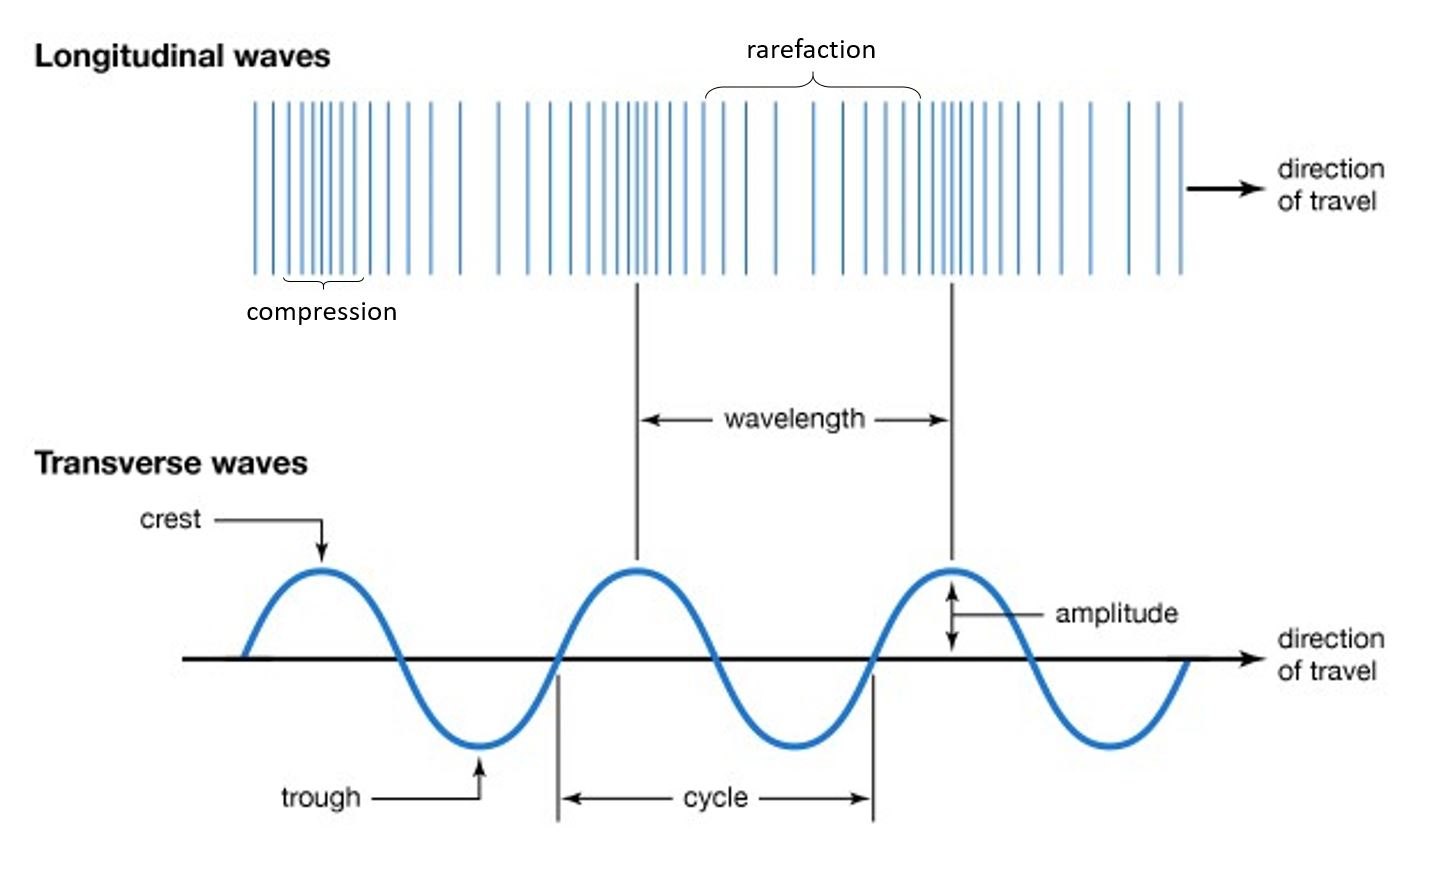
\includegraphics[scale=0.7]{notes/images/Waves-1.JPG}
        \caption{Longitudinal and Transverse waves}
    \end{figure}
    \FloatBarrier
\end{itemize}

\subsubsection{Characteristics of Periodic Waves}
A periodic wave is wave that can be represented by a periodic function of one-dimensional space that moves with constant speed. In this course, we'll typically represent this as a sinusoidal function. 
\begin{itemize}
    \item \textbf{Amplitude} ($A$) \\
    The maximum absolute value of a periodically varying quantity. In longitudinal waves it might be pressure or displacement from the equilibrium position. In a transverse wave it is displacement. In this course we will generally stick to the convention that amplitude is the maximum displacement from the equilibrium position.
    \item \textbf{Period} ($T$) \\
    The time between successive cycles of a wave. The time period can be calculated using 
    \begin{equation}
        T = \frac{t}{n},
    \end{equation}
    where $t$ is the time taken for $n$ cycles to occur. The unit of period is \textbf{seconds} ($s$)
    \item \textbf{Frequency} ($f$) \\
    The number of cycles per seconds, hence the frequency can be calculated using
    \begin{equation}
        f = \frac{n}{t},
    \end{equation}
    where $t$ is the time taken for $n$ cycles to occur. Thus frequency and time period are the reciprocal of one another, that is
    \begin{equation}
        f = \frac{1}{T} \text{ and } T = \frac{1}{f}.
    \end{equation}
    The unit of frequency is the \textbf{hertz} ($Hz$).
    \item \textbf{Phase} ($\phi$) \\
    Phase difference is said to be the difference in displacement of two points along the same wave or the difference in displacement of two points on different waves. The phase difference between two points on a wave separated by a distance of $x$ metres is given by 
    \begin{equation}
        \phi = \frac{x}{\lambda} 2\pi,
    \end{equation}
    where $\lambda$ is the wavelength of the wave. So phase is an angular quantity measured in \textbf{radians}.
    
    Two points are said to be \textbf{in phase} if they are separated by one complete cycle, that is if $\phi \pmod{2\pi} \equiv 0$, in a similar fashion, two points are said to be \textbf{out of phase} if they are separated by half a cycle, that is if $\phi \pmod{2\pi} \equiv \pi$. 
    \item \textbf{Wavelength} ($\lambda$) \\
    The distance between adjacent points in phase. In short, the wavelength is the length of one cycle. Wavelength is measured in \textbf{metres} ($m$).
    \item \textbf{Speed} ($v$) \\
    Waves propagate with a finite speed, sometimes called the wave speed, which has a number of factors:
    \begin{itemize}
        \item the type of wave
        \item the composition of the medium
        \item the state of the medium
    \end{itemize}
    From the definition of speed, it follows that the wave speed is the produce of frequency and wavelength for periodic waves, that is 
    \begin{equation}
        v = f \lambda.
    \end{equation}
    The unit for wave speed is the \textbf{metre per second} ($ms^{-1}$)
\end{itemize}

\subsection{Interference and Superposition}

For modelled by wave functions (we note that the functions themselves are irrelevant), if  $f_1(x, t)$ and $f_2(x,t)$ are waves, then so is
\begin{equation}
    f(x, t) = f_1(x, t) + f_2(x, t)
\end{equation}
which is called the \textit{superposition} of the waves $f_1$ and $f_2$. Waves add algebraically. This simple law is what gives rise to the fact that waves pass through each other without affecting each other. 

\begin{theorem}{(\textbf{Principle of Superposition})}
\textit{The principle of superposition states that when two waves meet at a point the resultant displacement at that point is equal to the sum of the displacements of the individual waves.}
\end{theorem}

Before giving an example of superposition, let us elaborate on the notation we introduced above. Waves can be modelled by linear displacement functions in the form $\vec{s} = f(x, t)$ where $\vec{s}$ is the displacement, the plot of a function of $x$ at a fixed time $t$ is known as the ``snapshot'' and the plot of a function of $t$ at fixed $x$ is the displacement of experienced by a particle $p$ at position $x$ as time passes.

Suppose $y_1$ and $y_2$ are waves with similar shapes, with $y_2$ traveling to the right, but $y_2$ traveling to the left and upside down. Then superposition is
\begin{equation*}
    y(x, t) = y_1(x, t) + y_2(x, t).
\end{equation*}
A snapshot at a fixed time $t$ looks like the plot below:
\begin{figure}[h!]
    \centering
    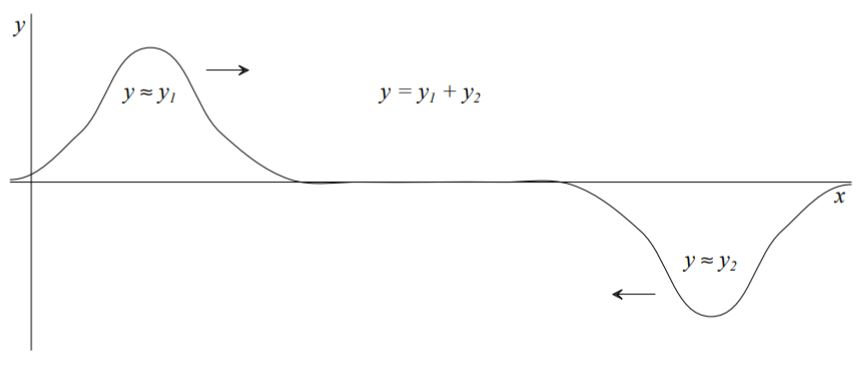
\includegraphics{notes/images/Superposition-1.JPG}
\end{figure}
\FloatBarrier
\noindent At some time $t_0$ later, the two waves will be exactly opposite, that is
\begin{equation*}
    y_1 (x, t_0) = -y_2(x, t_0)
\end{equation*}
and so $y(x, t_0) = 0$. At $t = t_0$, the snapshot is
\begin{figure}[h!]
    \centering
    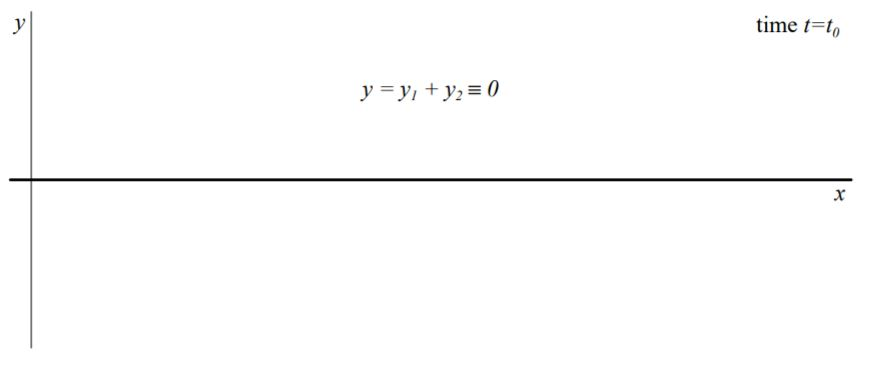
\includegraphics{notes/images/Superposition-2.JPG}
\end{figure}
\FloatBarrier
\noindent Somewhat later still, say at $t = t_1$, the waves have passed through each other, and the snapshot is
\begin{figure}[h!]
    \centering
    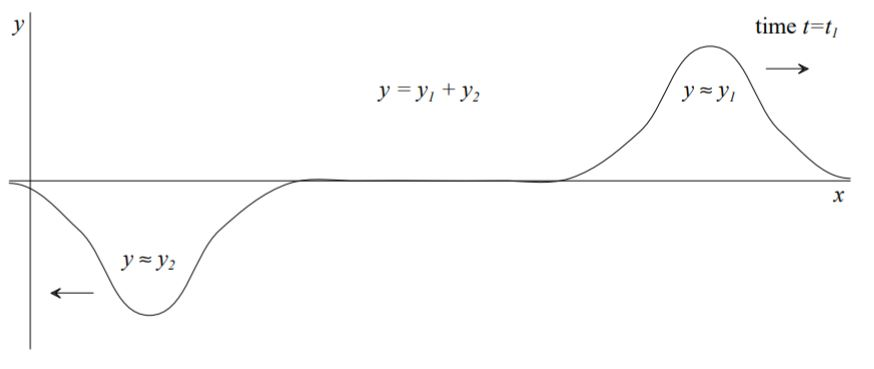
\includegraphics{notes/images/Superposition-3.JPG}
\end{figure}
\FloatBarrier

The superposition of these waves \textbf{interfere destructively}, that is when two waves superpose resulting in the cancellation of their displacement, i.e when the negative displacement of one wave coincides with the positive displacement of the other, which occurs when they are \textbf{antiphase}. The term \textbf{interfere} just refers to two waves superposing. The superposition of two waves that are in \textbf{phase} will \textbf{interfere constructively}, that is when two waves superpose resulting in a displacement with an increase amplitude. 

When two waves interfere, the intensity is affected. We will learn later on that $I_v \propto A^2$, where $I_v$ denotes intensity. In the case of constructive interference, an increase in intensity will occur which can be demonstrated by sounds  becoming ``louder'' and light becoming ``brighter''. The converse is true for destructive interference, that is a decrease in intensity will occur, i.e sounds are quieter and light is dimmer. 

\subsection{Diffraction and Reflection}

\textbf{Diffraction} is a property unique to waves; it is the bending or spreading of a wave around an obstacle or through an opening. The effects of diffraction are most apparent when the size of the obstacle or opening $a$ is approximately equal to the wavelength of the wave $\lambda$. This is why sound diffracts when it passes through a doorway, since the wavelength of the sound is similar to the width of the doorway. However, light has a much small wavelength, so it does not diffract through such a large gap. (See figure \ref{fig:diffraction-patterns}) 

\begin{figure}[h!]
    \centering
    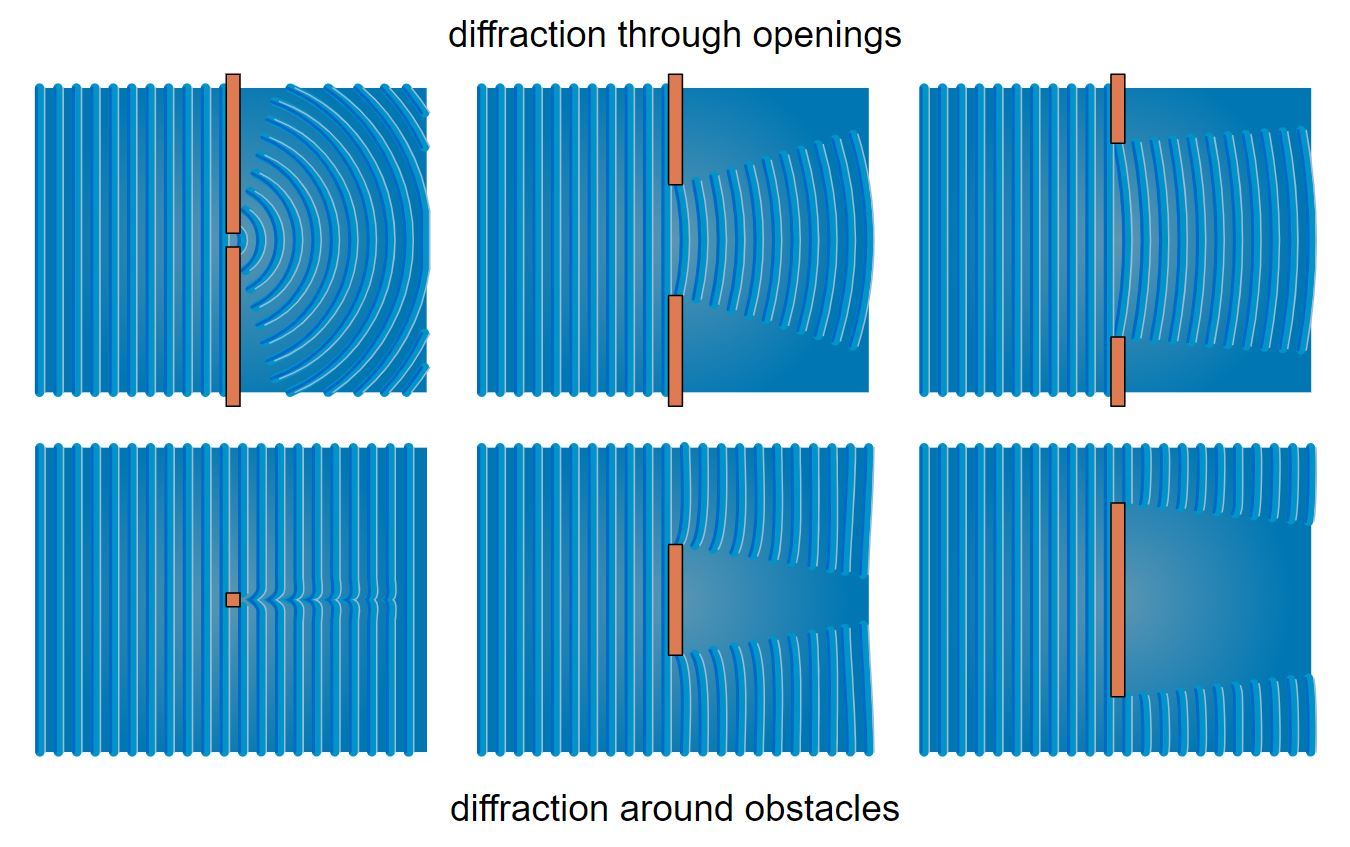
\includegraphics[scale=0.7]{notes/images/Diffraction-1.JPG}
    \caption{Diffraction Patterns}
    \label{fig:diffraction-patterns}
\end{figure}
\FloatBarrier

Typically when a wave travels through a medium and meets the boundary of another medium, it is \textbf{reflected}. The reflected wave does or does not undergo a phase change of $\pi$ radians depending on the boundary media. To describe this situation for strings, we will consider two cases where the boundary is fixed and where it is free to move. 

In the first case, suppose that one end of the string is tied to wall, as shown below. When the shape incidence from the left reaches the wall, the tension in the string tends to pull upwards on the wall. From Newton's third law, the reaction force exerted by the wall on the string is then downwards, making the reflected shape inverted thus undergoing a phase change of $\pi$ radians. 

\begin{figure}[h!]
    \centering
    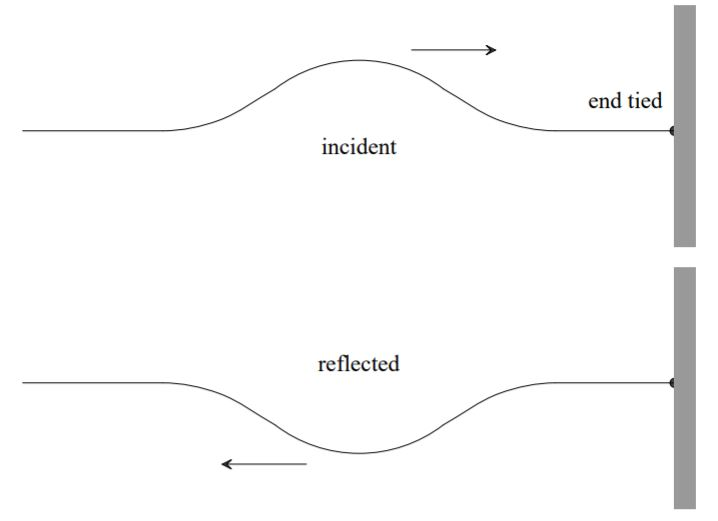
\includegraphics[scale=0.9]{notes/images/Reflection-1.JPG}
\end{figure}
\FloatBarrier

In the second case, the end of the string is tied to a frictionless ring, free to move up and down on a rod, as shown below. This time the pulse incident from the left just moves the ring upwards when it reaches the wall, making the reflected shape also upward, not inverted. 

\begin{figure}[h!]
    \centering
    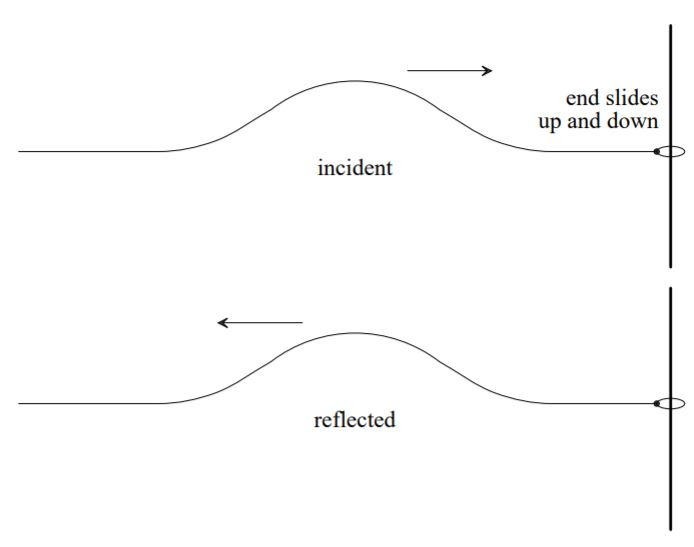
\includegraphics[scale=0.9]{notes/images/Reflection-2.JPG}
\end{figure}
\FloatBarrier

\begin{definition}{(\textbf{Law of Reflection})}
\textit{The law of reflection states the angle which the incident ray makes with the normal is equal to the angle which the reflected ray makes to the same normal. Mathematically, $\theta_i = \theta_r$.}
\begin{figure}[h!]
    \centering
    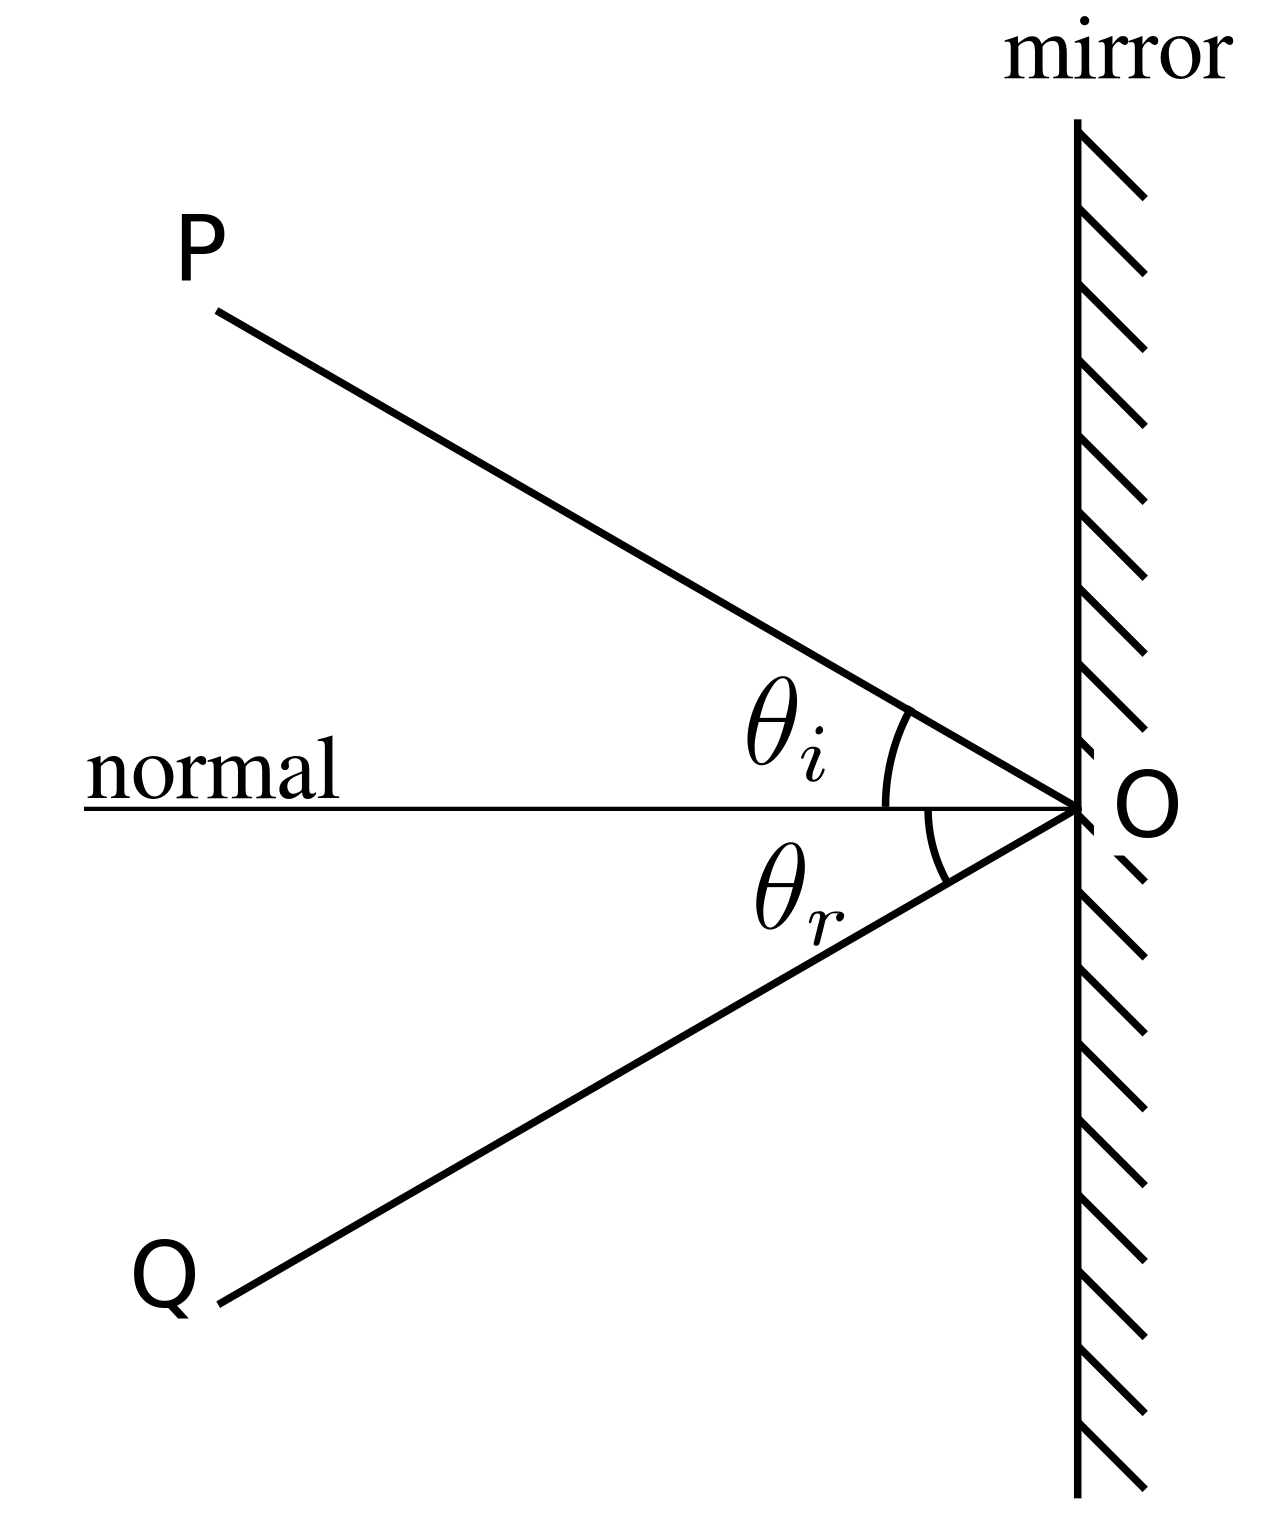
\includegraphics[scale=0.09]{notes/images/Law-Of-Reflection.JPG}
\end{figure}
\FloatBarrier

\end{definition}

\subsection{Polarization}

The phenomenon of \textbf{polarization} is something that only transverse waves exhibit. A wave in which the oscillations take place in a number of places is said to be \textbf{unpolarized}, while a wave in which the oscillations occur in one plane is \textbf{plane polarized} in that direction. Electromagnetic waves are transverse waves, and may be polarized. Unpolarized electromagnetic waves can be polarized using filters called \textbf{polarizers} or \textbf{polaroids}. A common use of polarizers is to prevent electromagnetic waves used in communications interfering with each other. 

\begin{figure}[h!]
    \centering
    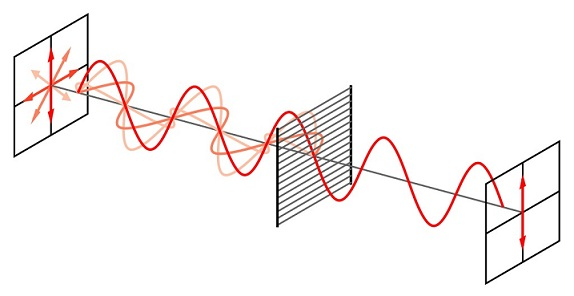
\includegraphics[scale=0.75]{notes/images/Polarization-1.JPG}
    \caption{A unpolarized and plane polarized wave}
\end{figure}
\FloatBarrier

\subsubsection{Malus' Law}

Suppose we have a second polaroid whose vertical makes an angle $\theta$ with the first one. The intensity of the wave that exits the second polaroid $I$ is given by
\begin{equation}
    I = I_0 \cos^2 \theta,
\end{equation}
where $I_0$ is the intensity of the wave exiting the first polaroid. 

\begin{figure}[h!]
    \centering
    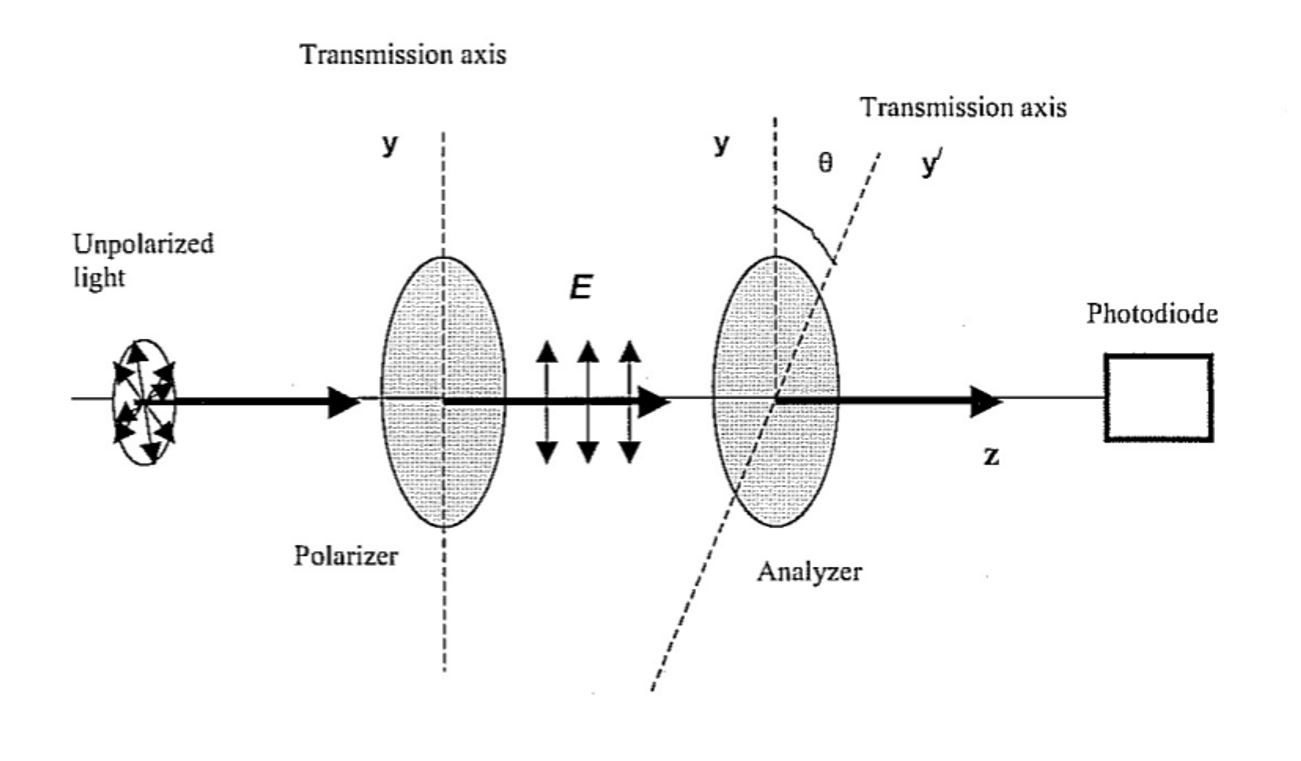
\includegraphics[scale=0.75]{notes/images/Malus-Law.JPG}
\end{figure}
\FloatBarrier

\subsection{Intensity}
\label{subsection:intensity}

The \textbf{intensity} $I_v$ of a wave is the time-averaged power $\langle P \rangle$ it transfers per unit of area $A$ through some region of space. The traditional way to indicate the time-average value of a varying quantity is to enclose it in the angled brackets $\langle \hspace{1mm} \rangle$. So the equation for intensity is
\begin{equation}
    I_v = \frac{\langle P \rangle}{A}
    \label{eq:intensity}
\end{equation}
measured in \textbf{watts per square metre} ($Wm^{-2}$). Intensity for \textit{mechanical waves} can be related to the density of the medium and the speed, frequency and amplitude of the wave via a long and horrible derivation. This equation or it's related derivation isn't required for A2 Physics, however, it will allow us to understand the factors that affect intensity. 

\begin{equation}
    I_v = 2 \pi^2 \rho f^2 v A^2,
\end{equation}
where $\rho$ denotes the density of the medium, $v$ is wave speed, $f$ is frequency and $A$ is amplitude. 

\subsubsection{Factors affecting mechanical waves}
\begin{itemize}
    \item $I_v \propto \rho$ \\
    The denser the medium, the more intense the wave. A dense medium packs more mass, since kinetic energy is proportional to mass, it follows that power is proportional to mass and therefore intensity is proportional to mass, thus rationalizing this relationship.
    \item $I \propto f^2$ \\
    The more cycles per unit of time, the more energy transferred. Therefore the more frequently a wave vibrates the medium, the more intense the wave is.
    \item $I \propto v$ \\
    The faster the wave travels, the more quickly it transmits energy. Since power is the rate of energy transferred, it follows that intensity is proportional to wave speed.
    \item $I \propto A^2$ \\
    Decreased amplitude means a reduced average speed of the oscillating \textit{particles} (considering the frequency is constant). Since kinetic energy is proportional to speed squared, it follows that intensity is directly proportional to the square of the amplitude. We should note that this is also implied by simple harmonic motion, since it's energy depends on the square of the oscillations amplitude. The relationship also applied to waves in general and therefore also applies to electromagnetic waves.
\end{itemize}

\subsubsection{Intensity and Distance}

Consider a circular wave, like the wave produced from dropping a stone in water, from a source. The wave carries energy with it which is spread over a larger and larger area as the wave spreads out. The radiant power from this wave is uniformly spread over the surface of a sphere with radius $r$. 

So the total radiant power $P$ at a distance $r$ from the source is spread over an area of a sphere $4\pi r^2$. Applying this to equation \ref{eq:intensity}, we have
\begin{equation}
    I_v = \frac{\langle P \rangle}{4 \pi r^2}.
\end{equation}
From this relationship, it follows that intensity is inversely proportional to the distance from the source.
\begin{equation}
    I_v \propto \frac{1}{r^2}.
\end{equation}

\section{Sound}

\subsection{Stationary Waves}

\textbf{Stationary waves}, also known as standing waves, refers to a wave that is \textit{not} progressive and a wave where the positions of the peaks and troughs are not moving. This is because a stationary wave is not a single wave, but the superposition of two progressive waves with the same frequency travelling in opposite directions. The easiest way to form the pair of progressive waves is by reflecting an incident wave at the boundary of media.

As they have the same frequency, at certain points they are in phase, forming \textbf{antinode}; an antinode is a point where the displacement is always at a maximum due to constructive interference.  At other points when the two waves are in antiphase, a \textbf{node} is formed - a point where the displacement is always zero (or at a minima). 

\begin{figure}[h!]
    \centering
    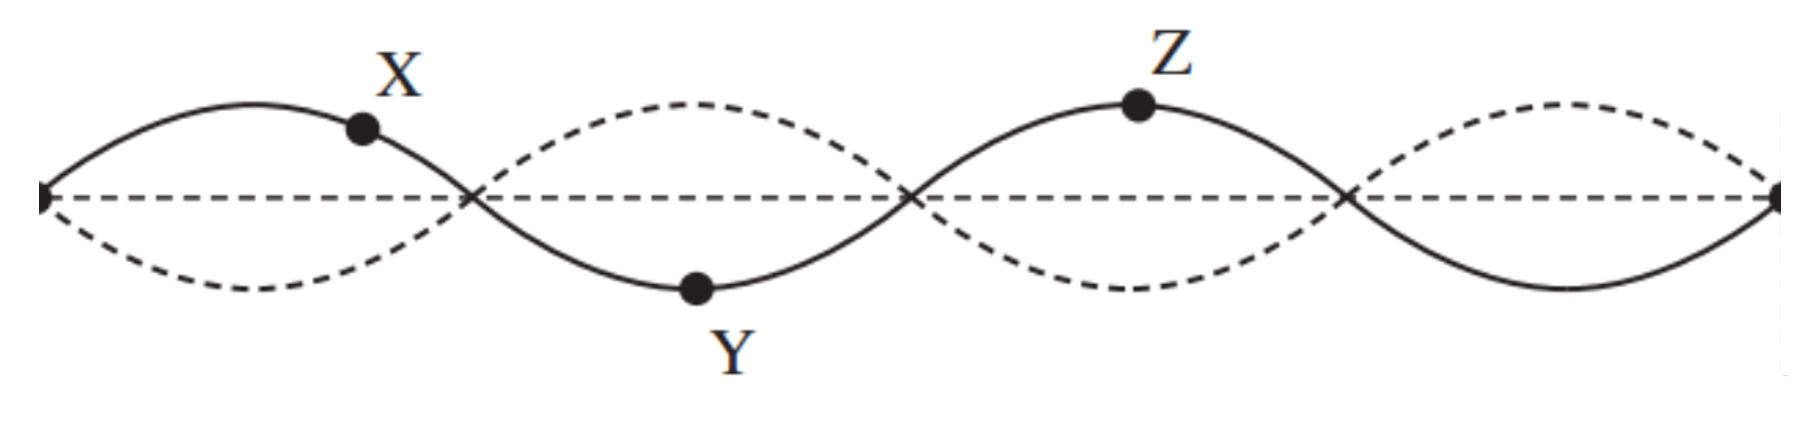
\includegraphics[scale=0.5]{notes/images/Stationary-Wave-Phase-Difference.JPG}
    \label{fig:stationary-wave}
    \caption{A stationary wave}
\end{figure}
\FloatBarrier

The separation between two adjacent nodes or antinodes is equal to half of the wave length of the original progressive wave and the frequency of the standing wave is equal to the frequency of the original progressive wave. 

\begin{table}[h!]
    {
        \begin{tabular}{l|p{0.4\linewidth}|p{0.4\linewidth}}
            \hspace{1mm} & Progressive wave & Stationary wave  \\
            \hline
            Energy transfer & Energy transferred in the direction of the wave. & No net energy transfer \\
            Wavelength & The distance in which the phase changes by $2\pi$ & Twice the distance between two adjacent nodes (or antinodes) is equal to the wavelength of the progressive wave that forms the stationary wave  \\
            Phase difference & The phase changes across one complete cycle of the wave & All parts of the wave between a pair of nodes are in phase, and on the other sides of the nodes they are in antiphase. For example, in figure \ref{fig:stationary-wave} the points X and Z are in phase, whereas X and Y are in antiphase. \\
            Amplitude & All peaks / troughs have the same amplitude (assuming no energy is lost) & Maximum amplitude occurs at antinodes
        \end{tabular}
    }
\end{table}
\FloatBarrier

\subsection{Harmonics}

Any system in which stationary waves can form has numerous frequencies in which a stationary wave can form. The set of all possible stationary waves are known as the \textbf{harmonics} of a system. The simplest of the harmonics is called the \textbf{fundamental} or \textbf{first harmonic}, which has an associated \textit{fundamental} frequency denoted $f_0$ or $f$. Subsequent stationary waves called the second harmonic, third harmonic, etc whose frequencies are multiples of the fundamental frequency, that is the second harmonic has a frequency of $2f_0$, the third harmonic has a frequency of $3f_0$, etc. So what wavelengths will form stationary waves in a simple, one-dimensional system with these frequencies? There are three simple cases  

In the first case, suppose that a medium is bounded such that its opposite ends can be considered fixed, it follows that nodes will then form at the ends. The simplest stationary wave that can form under these circumstances has one antinodes in the middle. The distance between the bounds is half a wavelength. The same argument can be applied to the second harmonic, finding the distance between the bounds is a wavelength. It should become obvious that a pattern begins to emerge (see figure \ref{fig:harmonic-1}), that is for the $n^{th}$ harmonic with frequency $nf$ the wavelength is given by $\lambda = \frac{2}{n} L$, where $L$ is the distance between the bounds.  

\begin{figure}[h!]
    \centering
    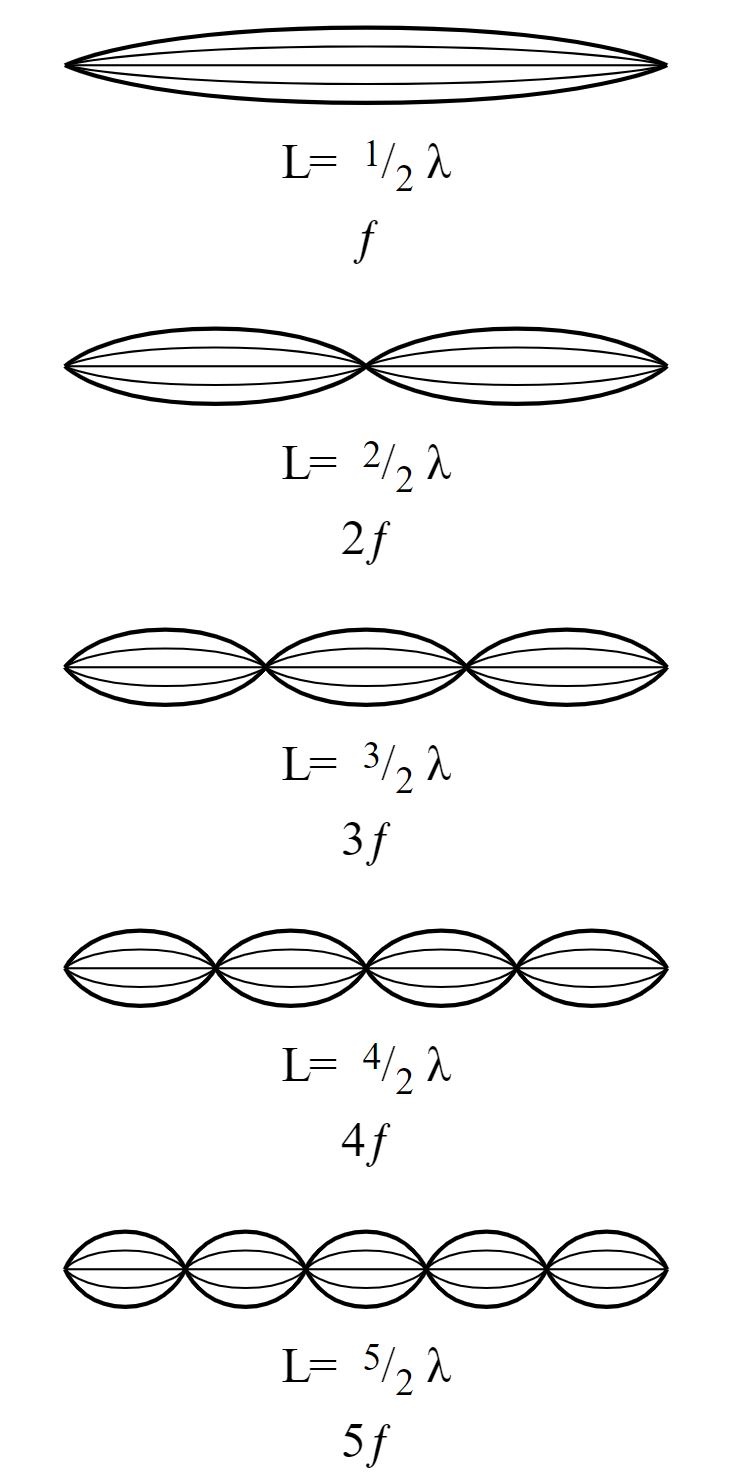
\includegraphics[scale=0.5]{notes/images/Harmonic-1.JPG}
    \caption{Harmonics with fixed ends}
    \label{fig:harmonic-1}
\end{figure}
\FloatBarrier

In the second case, suppose that a medium is bounded such that its opposite ends can be considered free, so antinodes will form at the ends. The simplest stationary wave that can form under these circumstances has one node in the middle. The distance between the bounds is half the wavelength. To make the next possible stationary wave, place another antinode in the center. We now have one whole wavelength. It should become apparent that we will get the same relationships for the stationary waves formed between two free ends that we have for two fixed ends. The only difference is that nodes are replaced with antinodes and vice versa. So for the $n^{th}$ harmonic with frequency $nf$ the wavelength is given by $\lambda = \frac{2}{n} L$, where $L$ is the distance between the bounds. 

\begin{figure}[h!]
    \centering
    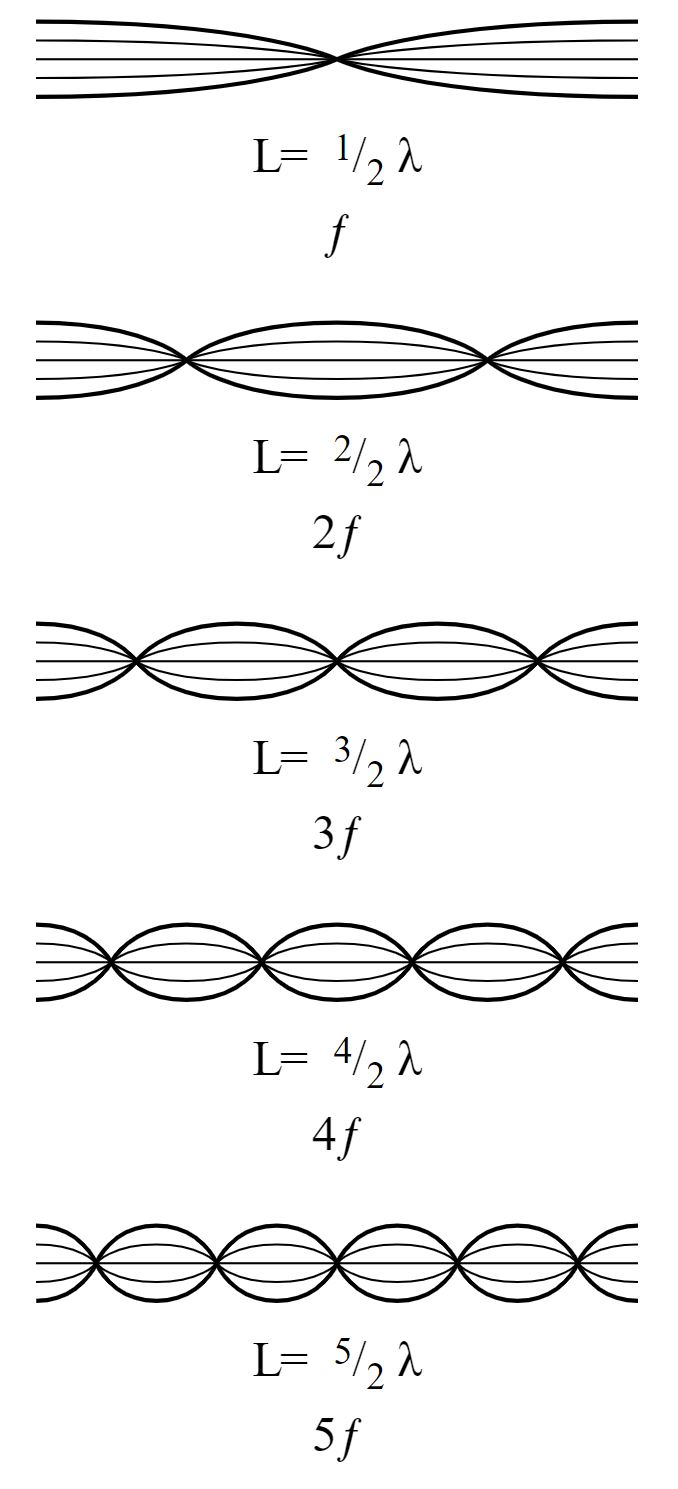
\includegraphics[scale=0.5]{notes/images/Harmonic-2.JPG}
    \caption{Harmonics with free ends}
\end{figure}
\FloatBarrier

In the third and final case, suppose that a medium has one fixed end and one free end. A node will always form at the fixed end while an antinode will always form at the free end. The simplest stationary wave that can form under these conditions has a wavelength that is 4 times the distances between the bounds. The next possible stationary wave is formed by adding a node and an antinode, with wavelength that is four thirds of the distance between the bounds. Repeating this procedure, we begin to notice a pattern; for the $n^{th}$ harmonic with frequency $nf$ the wavelength is given by $\lambda = \frac{4}{n} L$. However, we note that the frequencies of the harmonics are always odd multiples of the fundamental frequency and therefore we can only have odd harmonics, that is $n \in \mathbb{Z}_{odd}^+$

\begin{figure}[h!]
    \centering
    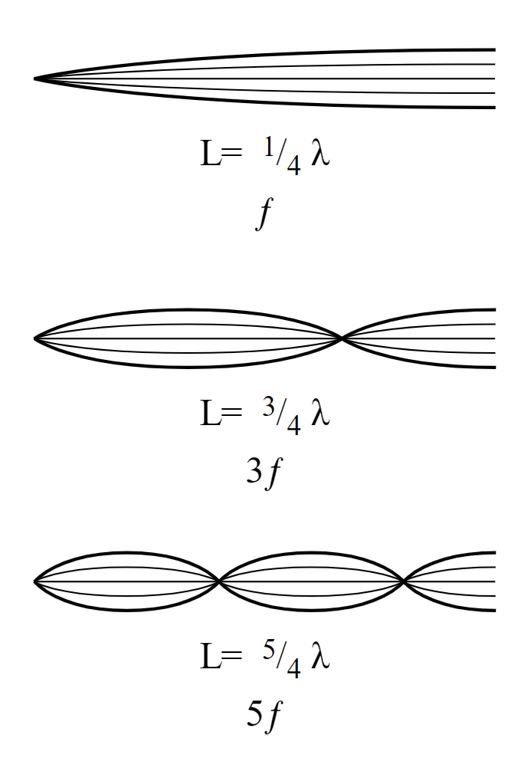
\includegraphics[scale=0.55]{notes/images/Harmonic-3.JPG}
    \caption{Harmonics with one fix end and one free end}
\end{figure}
\FloatBarrier

\section{Optics}

\subsection{Electromagnetic Waves}
\label{subsection:electromagnetic-waves}

As stated in section \ref{subsection:nature-of-waves}, electromagnetic (EM) waves are those waves in which electric and magnetic fields are perpendicular to each other as well as the direction of propagation and requires no medium. 

\noindent The properties of EM waves are as follows:
\begin{itemize}
    \item These waves are transverse in nature
    \item These waves propagate through a vacuum with the speed of light
    \item The speed squared of an electromagnetic wave is given by 
    \begin{equation}
        c^2 = \frac{1}{\varepsilon_0 \mu_0},
    \end{equation}
    where $\varepsilon_0$ is the permittivity of a vacuum and $\mu_0$ is the permeability of a vacuum.
    \item The oscillating electric and magnetic fields are self sustaining if they are perpendicular to one another and the direction of propagation, and are in phase.
\end{itemize}

\begin{figure}[h!]
    \centering
    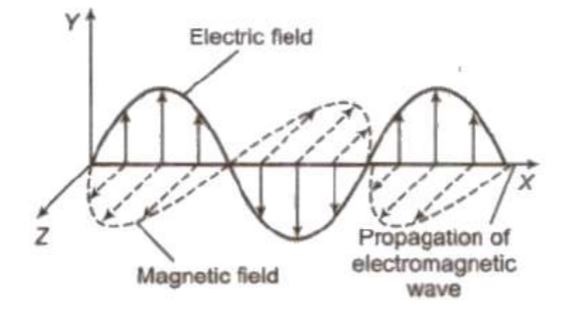
\includegraphics{notes/images/EM.JPG}
    \caption{An EM wave}
\end{figure}
\FloatBarrier

\subsubsection{The Electromagnetic Spectrum}

The arranged array of electromagnetic radiations in the sequence of their wavelength of frequency is called the \textbf{electromagnetic spectrum} and ranges from \textbf{radio waves} with the longest wavelength to \textbf{gamma rays} with the shortest wavelength. 

\begin{figure}[h!]
    \centering
    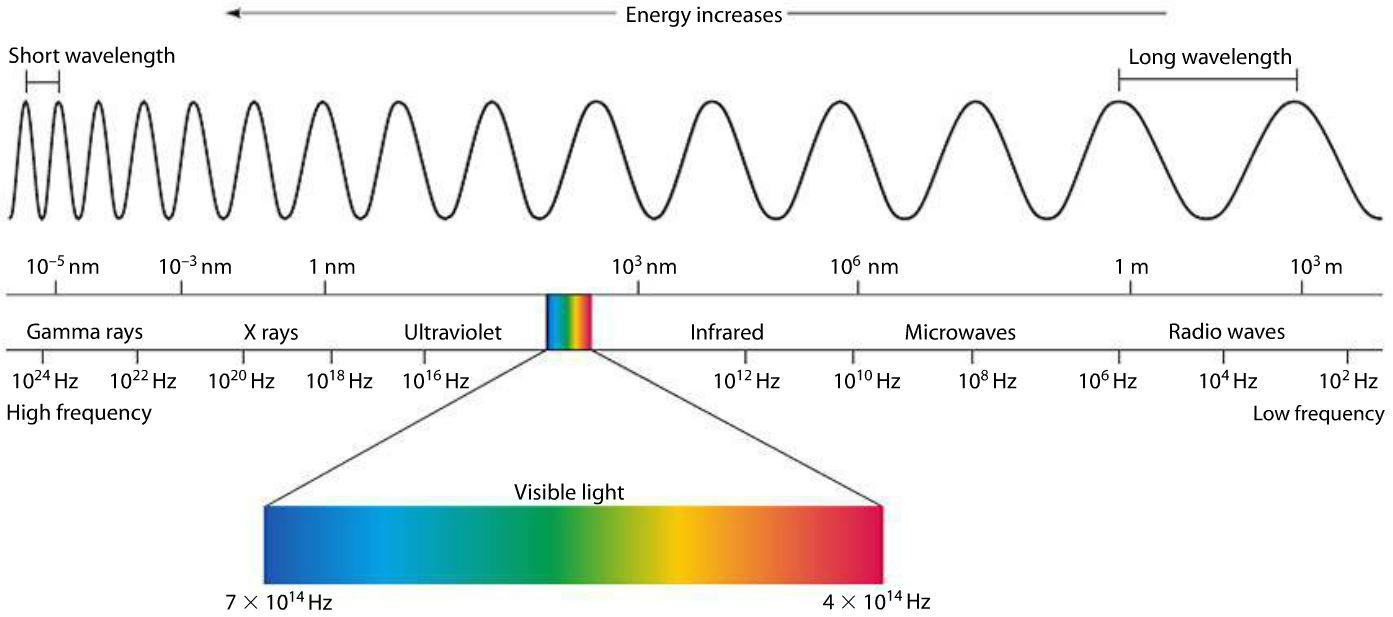
\includegraphics[scale=0.4]{notes/images/EM-Spectrum.JPG}
    \caption{The electromagnetic spectrum}
\end{figure}
\FloatBarrier

\subsection{Refraction}

\textbf{Refraction} occurs when a wave changes direction at the boundary of media. This is due to a change in wavespeed when passing from one medium to another. 

If the wave slows down it will refract towards the normal, whereas if the wave speeds up it refracts away from the normal, as shown below.


\begin{figure}[h!]
    \centering
    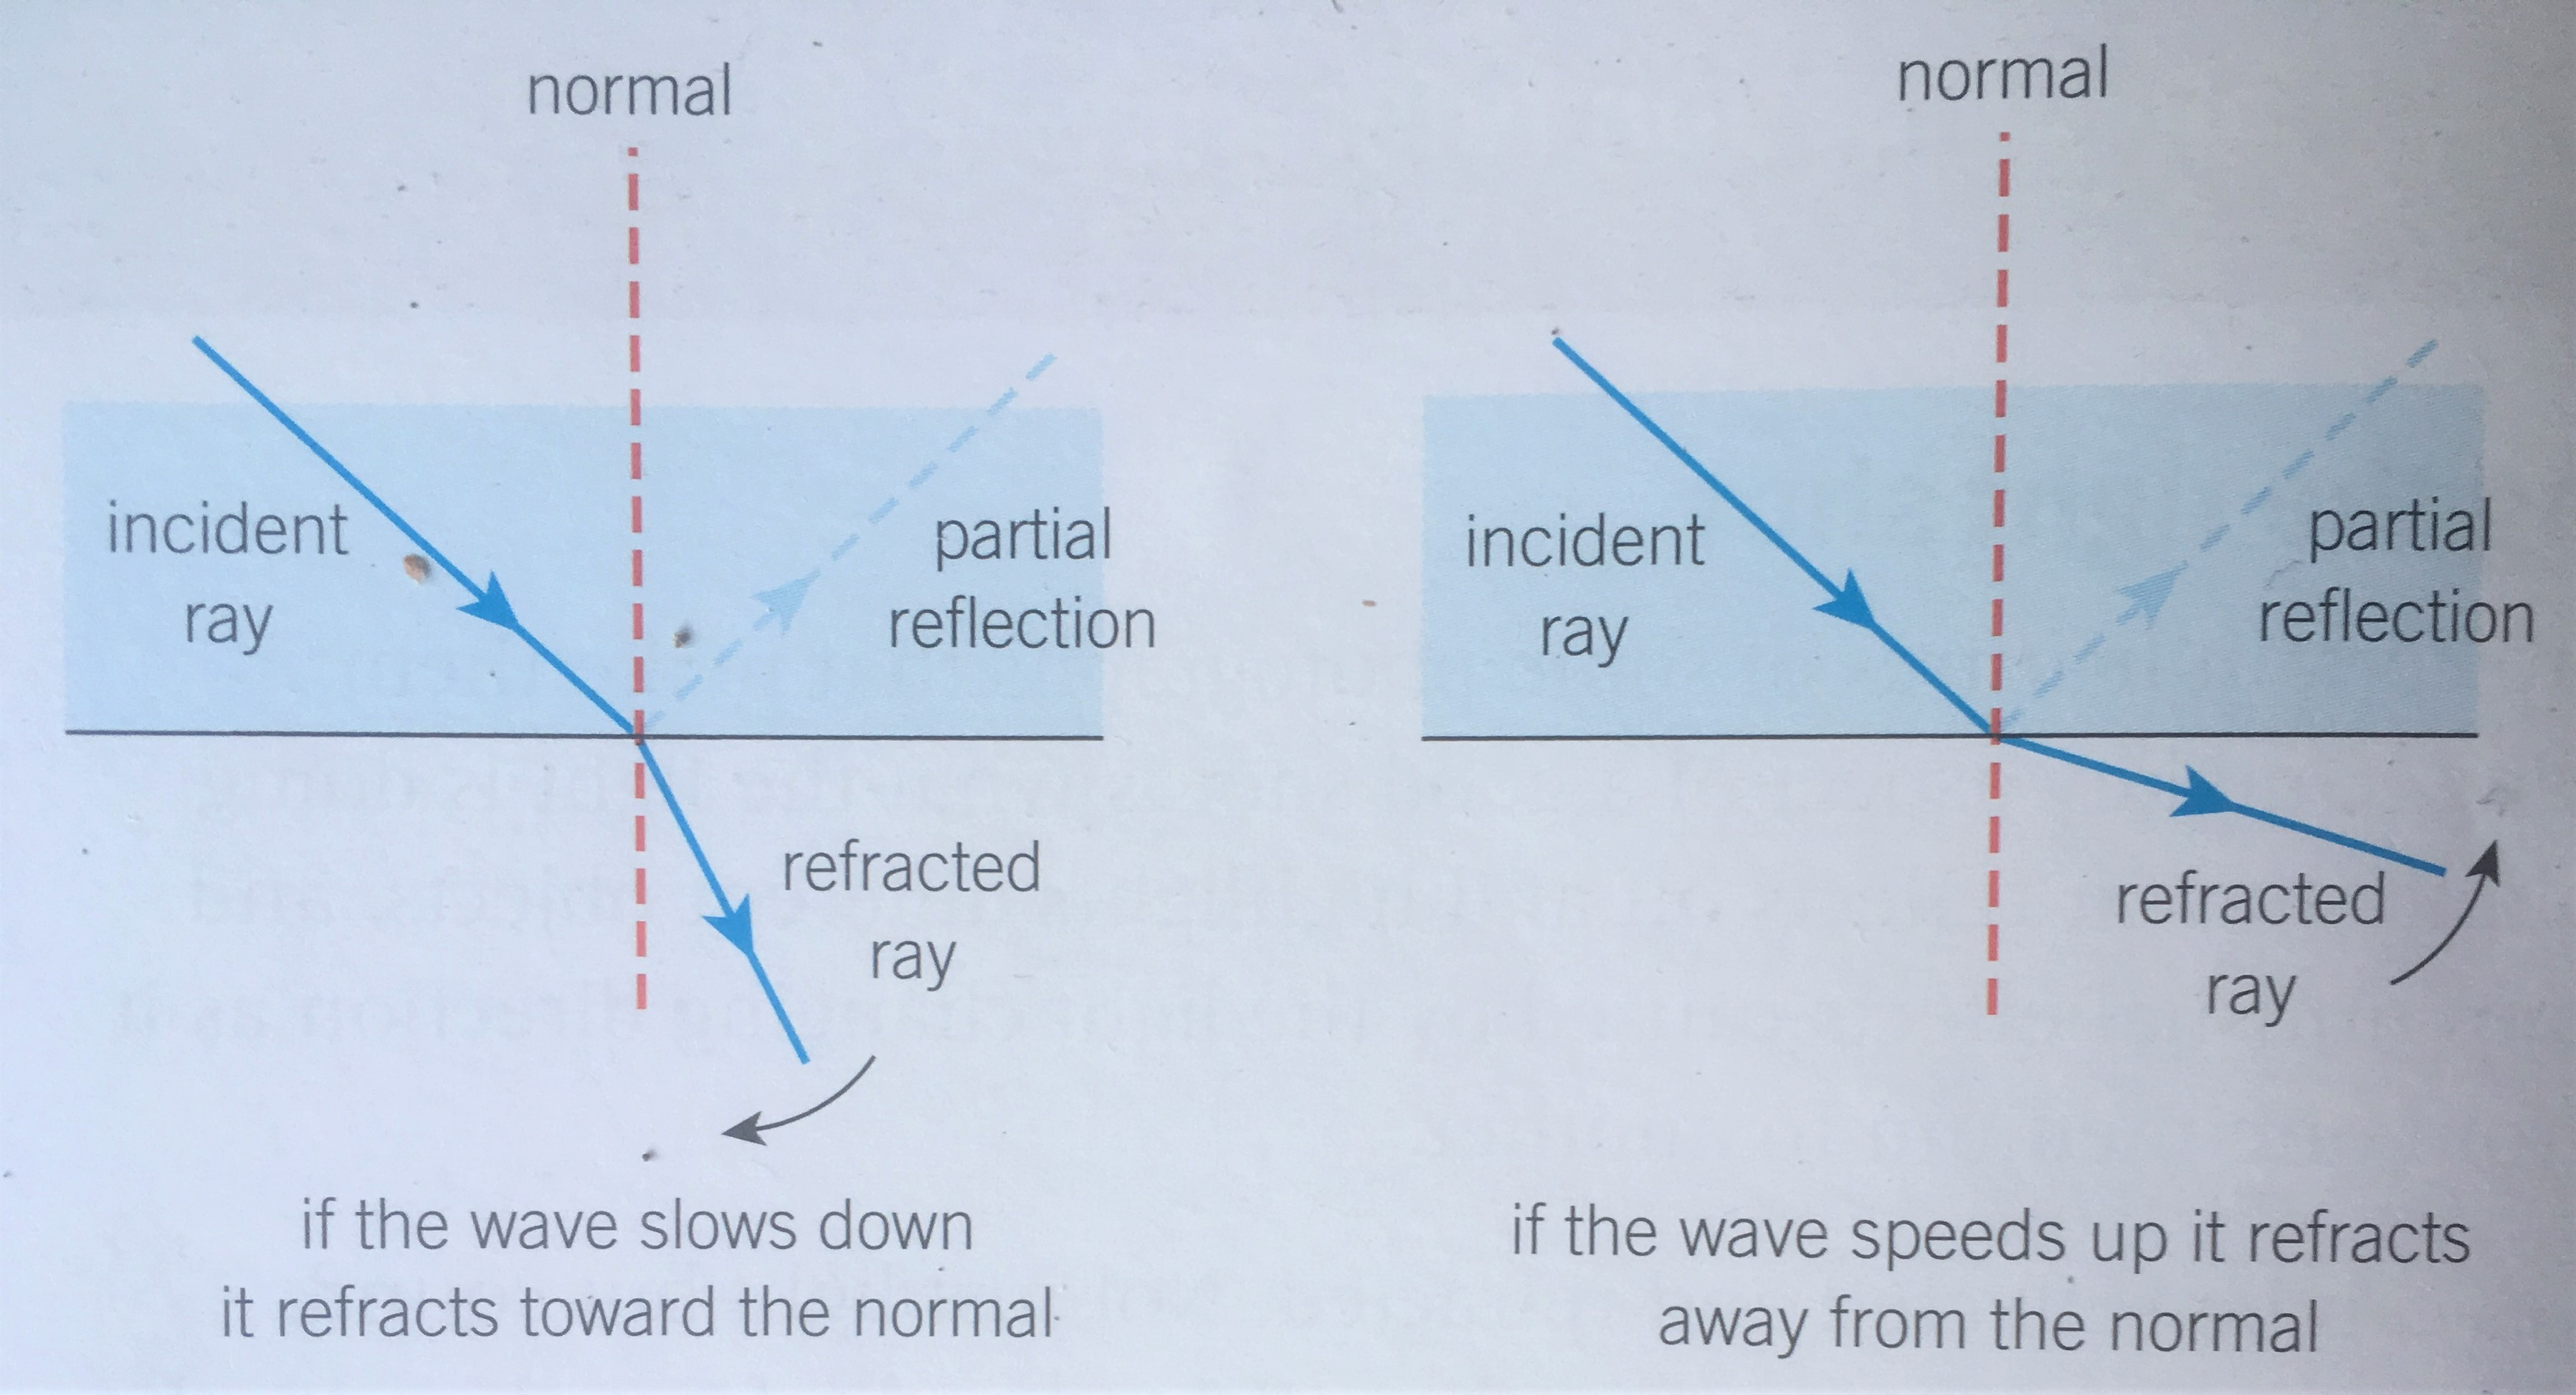
\includegraphics[scale=0.09]{notes/images/Refraction-2.JPG}
\end{figure}
\FloatBarrier


Snell's law (named after Willebrord Snellius) describes the relationship between the angles of incidence and refraction. The law states that the ratio of the sines of the angles of incidence and refraction is equivalent to the ratio of the velocities, wavelengths or equivalent to the reciprocal of the ratios of indices of refraction, that is:
\begin{equation}
    \frac{\sin \theta_1}{\sin \theta_2} = \frac{n_2}{n_1} = \frac{v_1}{v_2} = \frac{\lambda_1}{\lambda_2}. 
\end{equation}

\begin{figure}[h!]
    \centering
    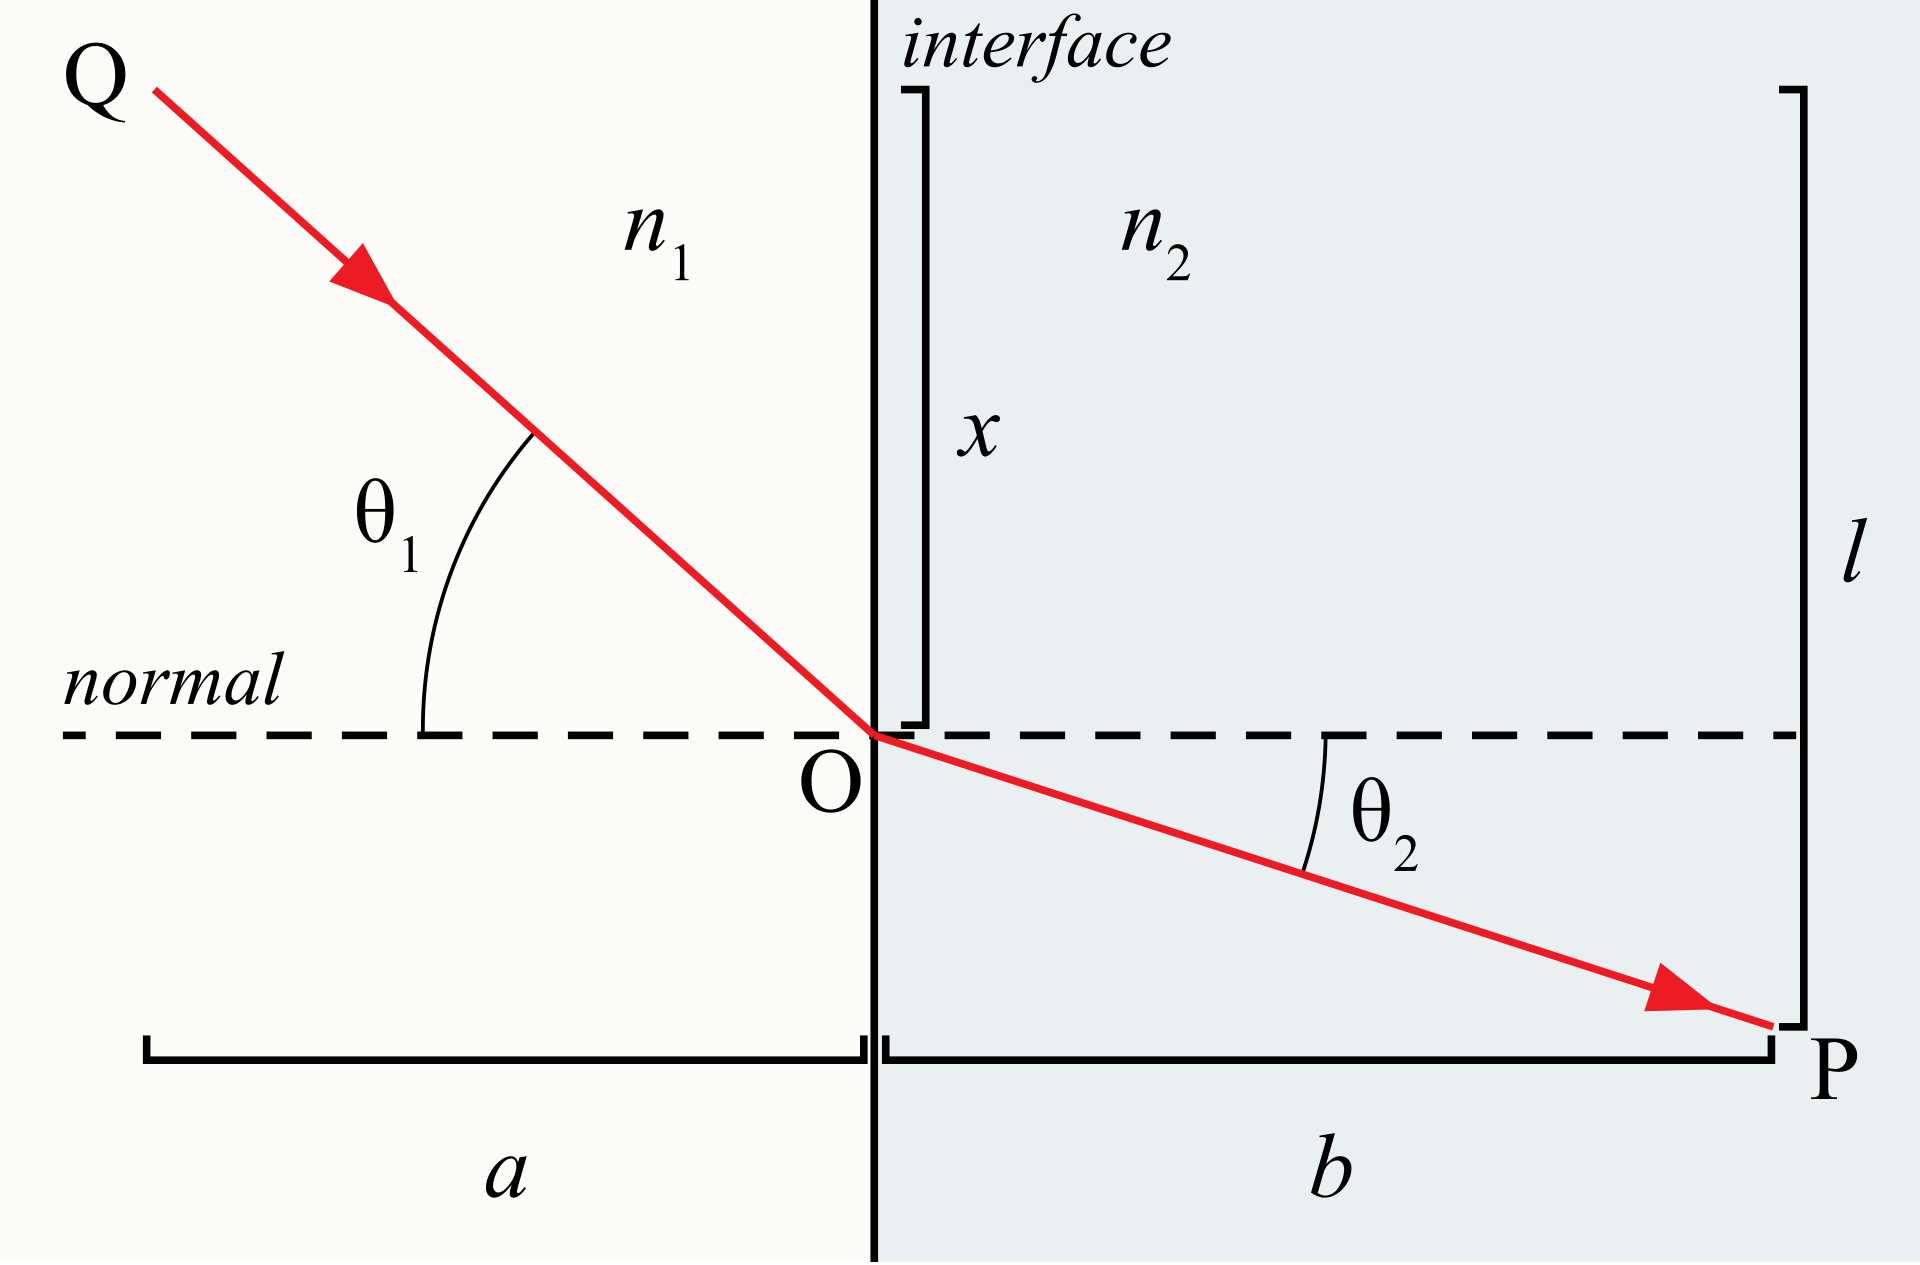
\includegraphics[scale=0.1]{notes/images/Snells-Law.JPG}
    \caption{Snell's Law Diagram}
\end{figure}
\FloatBarrier

We will now consider a special case of refraction, known as \textbf{total internal reflection} (TIR) of light at the boundary of two different media. The following conditions must be met in order for TIR to occur
\begin{itemize}
    \item Light must be travelling in a medium that has a higher refractive index than the boundary medium.
    \item The angle of incidence must be greater than the \textbf{critical angle} denoted $C$. The critical angle is dependent on the refractive indices of the media.
    \begin{figure}[h!]
        \centering
        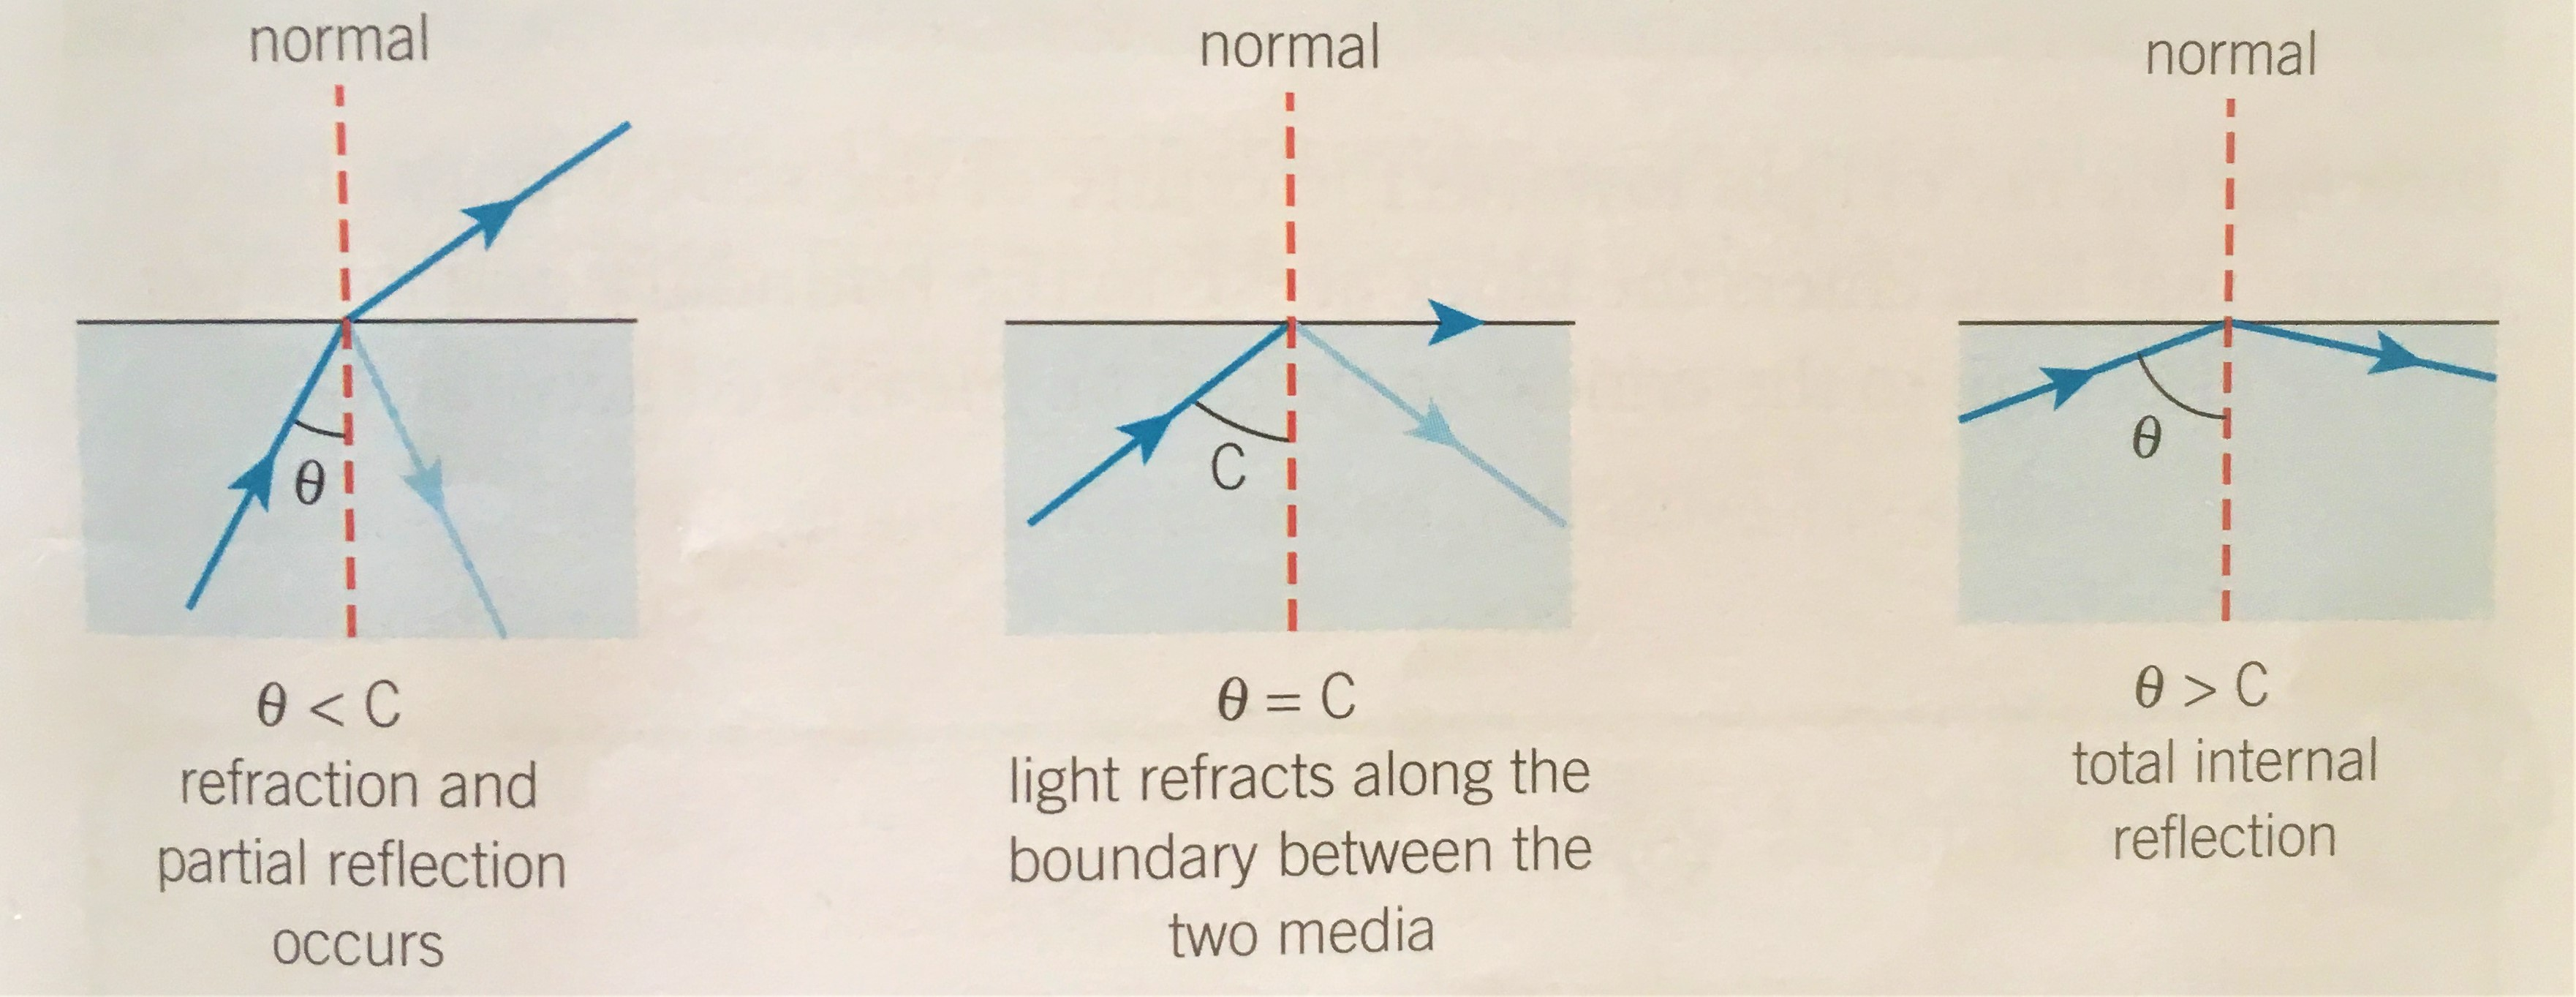
\includegraphics[scale=0.1]{notes/images/Critical-Angle.JPG}
    \end{figure}
    \FloatBarrier
    From Snell's law is follows that $n_1 \sin \theta_1 = n_2 \sin \theta_2$. Given $\theta_2 = \pi / 2$, we have $n_1 \sin C = n_2$, which yields:
    \begin{equation}
        \sin C = \frac{n_2}{n_1} = \frac{v_1}{v_2} = \frac{\lambda_1}{\lambda_2}. 
    \end{equation}
\end{itemize}



\subsection{Interference Patterns of Light}

Consider two waves. At certain points these superposed waves are in phase, interfering constructively, or out of phase, causing destructive interference. Most waves do not form a \textit{stable} interference pattern but one that changes all the time. In order to form a stable interference pattern, the incident waves must be \textbf{coherent}. This means that the waves from the sources must maintain a constant phase relation. For example, if two waves are in anti-phase, that is $\phi = \pi$, then this phase difference must not change with time to achieve a constant phase relation. 

Interference patterns contain a series of \textbf{minima} and \textbf{maxima}, where constructive and destructive interference occurs, respectively. Minima and maxima are a result of the two waves having travelled difference distances from their sources. This difference in the distance travelled is called the \textbf{path difference}, we will analyze these path differences mathematically to find criteria for the minima and maxima. 

Let us points $S_1$ and $S_2$ which serve as the sources of coherent waves. The waves emerging from the two sources then interfere and form an interference pattern. The points of maximum intensity correspond to maxima, and the converse is true for minima. Figure \ref{fig:interference-at-points} shows the ways in which the waves could combine to interfere constructively or destructively. 

\begin{figure}[h!]
    \centering
    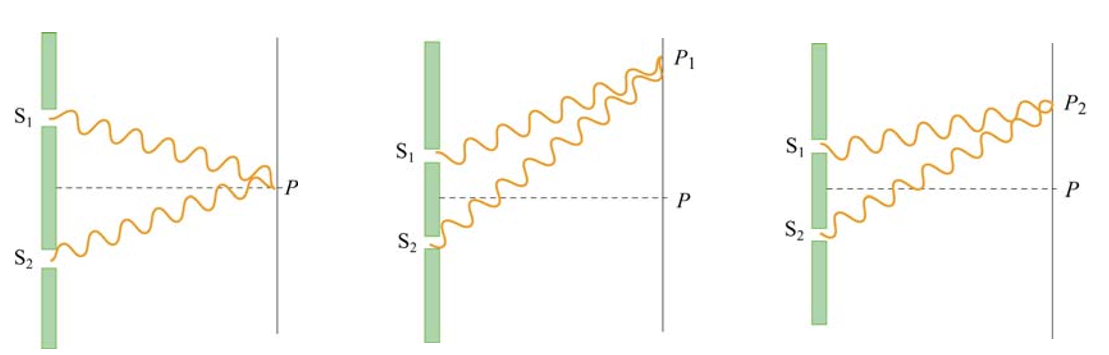
\includegraphics[scale=0.5]{notes/images/Interference-Two-Source-1.JPG}
    \caption{Constructive interference at $P$ and $P_1$. Destructive interference at $P_2$}
    \label{fig:interference-at-points}
\end{figure}
\FloatBarrier

The geometry of this interference pattern is shown below

\begin{figure}[h!]
    \centering
    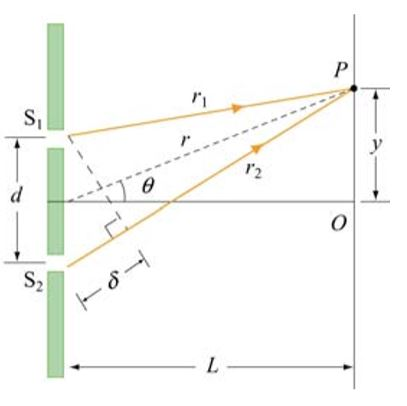
\includegraphics[scale=0.6]{notes/images/Interference-Two-Source-2.JPG}
    \caption{Two source experiment}
\end{figure}
\FloatBarrier

Consider a point $P$ where the two waves interfere, with a distance $y$ from the point $O$ that lies on a line perpendicular to the distance $L$ from the two source system. The wave from source 2 will travel an extra distance of $\delta = r_2 - r_2$ to the point $P$ than the wave from source 1. This extra distance is the \textit{path difference}. From the figure above, we have, using the law of cosines, 
\begin{equation}
    \label{eq:derivation-interference-1}
    r_1^2 = r^2 + \left(\frac{d}{2}\right)^2 - dr\cos \left(\frac{\pi}{2} - \theta\right) = r^2 + \left(\frac{d}{2}\right)^2 -dr \sin \theta
\end{equation}
and
\begin{equation}
    \label{eq:derivation-interference-2}
    r_2^2 = r^2 + \left(\frac{d}{2}\right)^2 - dr\cos \left(\frac{\pi}{2} + \theta\right) = r^2 + \left(\frac{d}{2}\right)^2 -dr \sin \theta
\end{equation}
Subtracting equation \ref{eq:derivation-interference-1} from equation \ref{eq:derivation-interference-2} yields:
\begin{equation*}
    r_2^2 - r_2^2 = (r_2 + r_1)(r_2 - r_1) = 2dr \sin \theta 
\end{equation*}
In the limit of $L \gg d$ (i.e. the distance to the screen is much greater than the distance between the sources), the sum of $r_2$ and $r_2$ may be approximated by $r_1 + r_2 \approx 2r$, and the path difference becomes
\begin{equation*}
    \delta = r_2 - r_1 \approx d \sin \theta 
\end{equation*}
In this limit, the two waves $r_1$ and $r_2$ are essentially treated as being parallel, as shown below

\begin{figure}[h!]
    \centering
    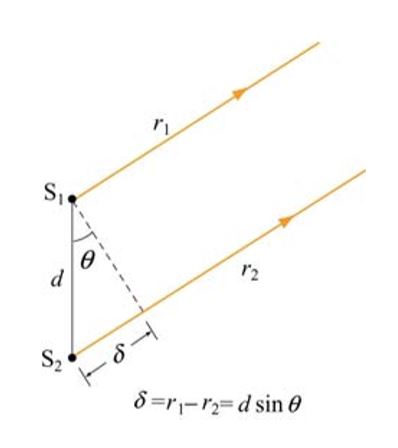
\includegraphics[scale=0.5]{notes/images/Interference-Two-Source-3.JPG}
    \caption{Path difference between the two waves, assuming $L \gg d$.}
\end{figure}
\FloatBarrier

Whether the two waves are in phase or out of phase is determined by the value of $\delta$. Constructive interference occurs when $\delta$ is zero or an integer multiple of the wave length $\lambda$:
\begin{equation}
    \label{eq:path-difference-constructive}
    \delta = d \sin \theta = n \lambda, \hspace{5mm} n = 0, \pm 1, \pm 2, \pm 3, \ldots
\end{equation}
where $n$ is called the \textit{order number}. The zeroth-order maximum corresponds to the central maxima, and the first-order maxima are the points of constructive interference either side of the central maxima, and so on.

On the other hand, when $\delta$ is equal to an odd integer multiple of $\lambda / 2$, the waves will be $\pi$ radians out of phase (i.e. anti-phase) at $P$, resulting in destructive interference. Hence the condition for destructive interference is given by
\begin{equation}
    \label{eq:path-difference-destructive}
    \delta = d \sin \theta = \left(n - \frac{1}{2}\right) \lambda, \hspace{5mm} n = \pm 1, \pm 2, \pm 3, \ldots
\end{equation}

In the figure below, we show how a path difference of $\lambda / 2$ results in a destructive interference and a path difference of $\lambda$ leads to constructive interference. 
\begin{figure}[h!]
    \centering
    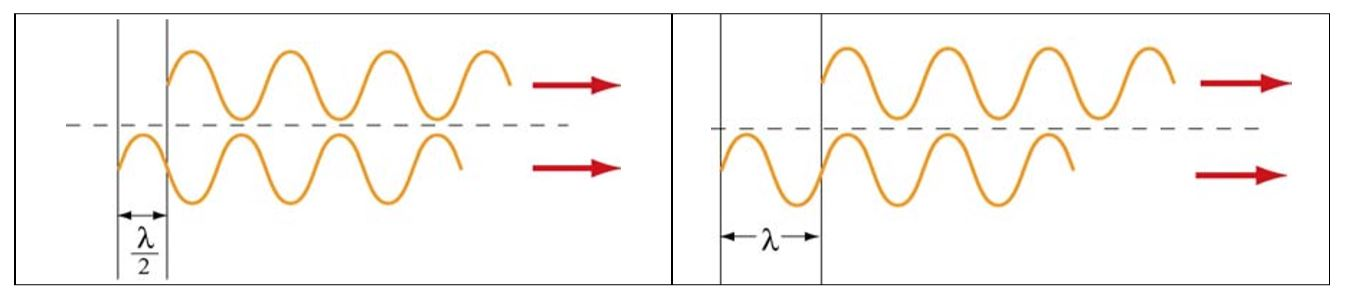
\includegraphics[scale=0.4]{notes/images/Interference-Two-Source-4.JPG}
    \caption{Destructive interference (left) and constructive interference (right).}
\end{figure}
\FloatBarrier
\noindent From the path difference, we can also deduce the phase difference between points on the waves using 
\begin{equation*}
    \phi = \frac{x}{\lambda} 2 \pi,
\end{equation*}
and substituting $\delta$ for $x$ in the equation above; yielding a phase difference for the central maxima of zero radians, $\pi$ radians for the first-order minima, $2\pi$ radians for the first-order maxima, $3\pi$ radians for the second-order minima, and so on.  The path differences and phase differences for a typical two source interference pattern are shown in the figure below

\begin{figure}[h!]
    \centering
    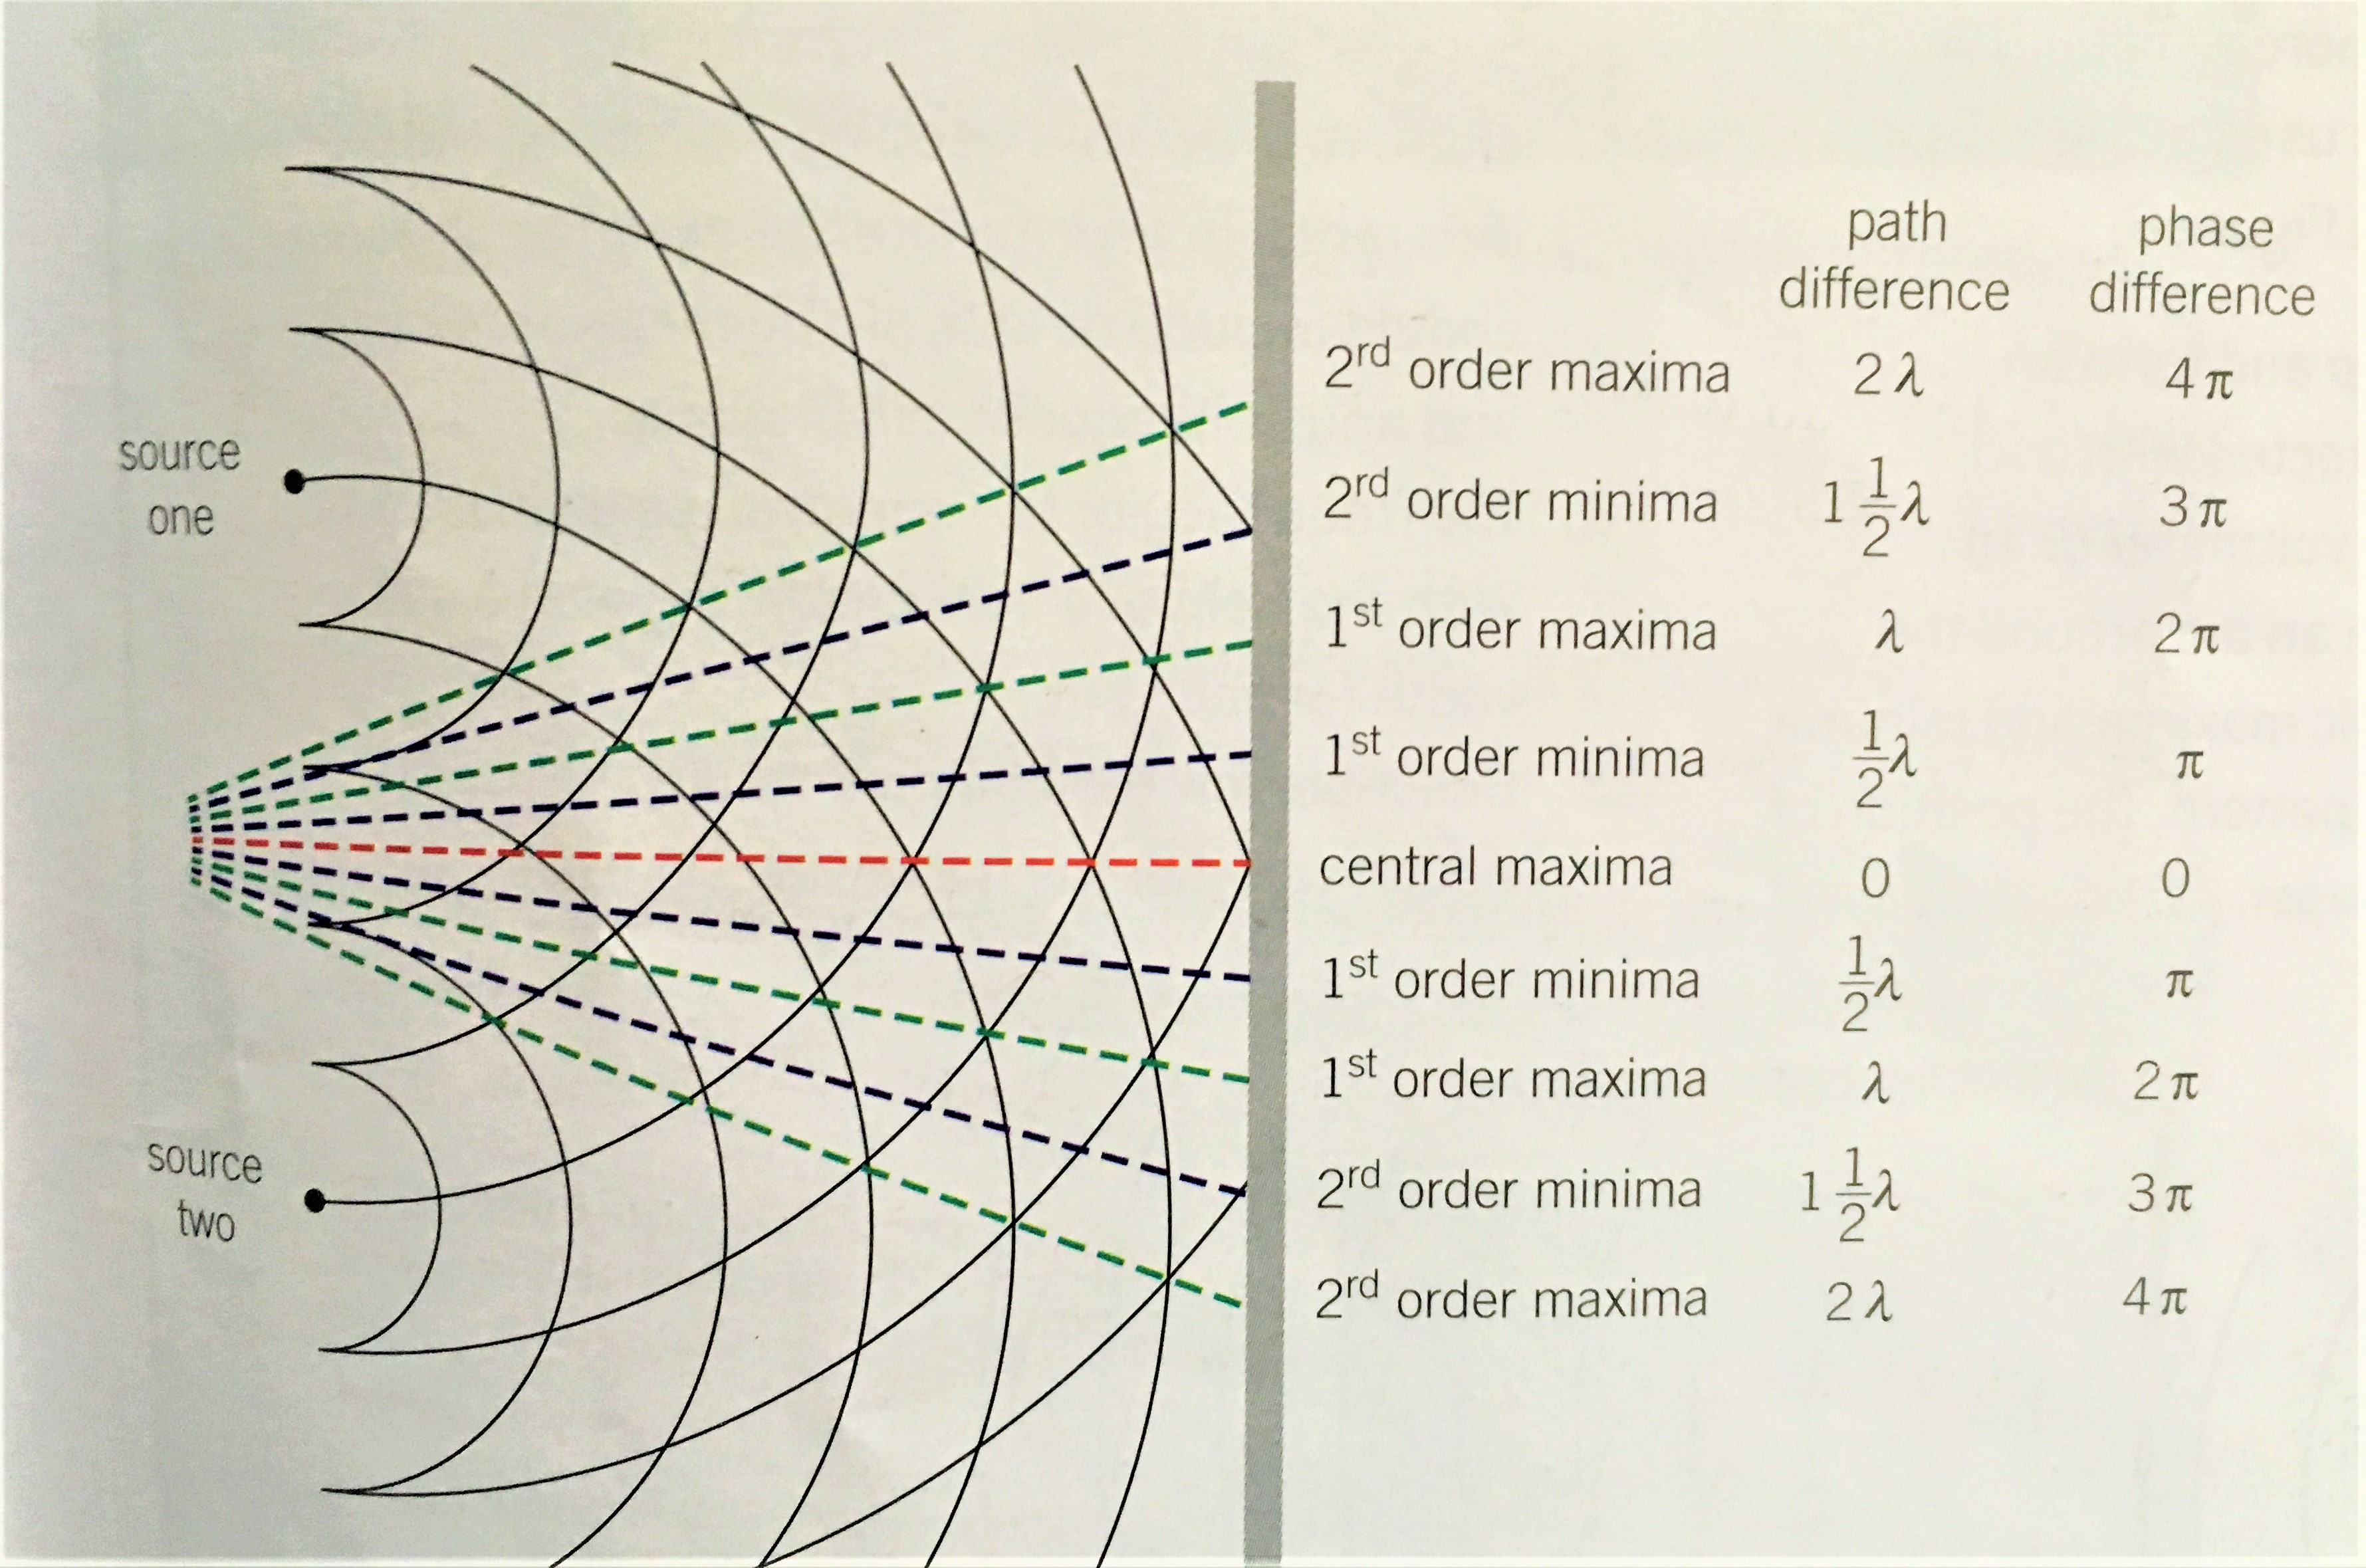
\includegraphics[scale=0.1]{notes/images/Interference.JPG}
    \caption{Two source wave interference pattern}
\end{figure}
\FloatBarrier

\subsection{Young's Double-Slit Experiment}

In 1801 Thomas Young carried out an experiment in which the wave nature of light was demonstrated. Two coherent waves are needed to form an interference pattern (as discussed above), Young devised a method to achieve this that now bears his name. He used a \textbf{monochromatic} source of light (which can be achieved by using a colour filter that allows only a specific frequency of light to pass) and a narrow single slit $S_0$ to diffract the light. The emerging light then arrives at the second screen which has two parallel slits $S_1$ and $S_2$ in phase. The two slits then serve as the sources of coherent light, with the emerging light waves interfering with each other to form an interference pattern on the viewing screen, The bright bands (fringes) correspond to maxima and the dark bands are minima; as shown below.
\begin{figure}[h!]
    \centering
    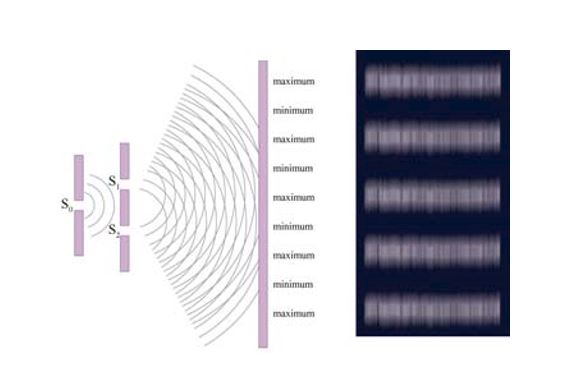
\includegraphics[scale=0.7]{notes/images/Interference-Single-Source-1.JPG}
    \caption{Young's double-slit experiment.}
\end{figure}
\FloatBarrier

The geometry of the double-slit interference experiment is shown below.
\begin{figure}[h!]
    \centering
    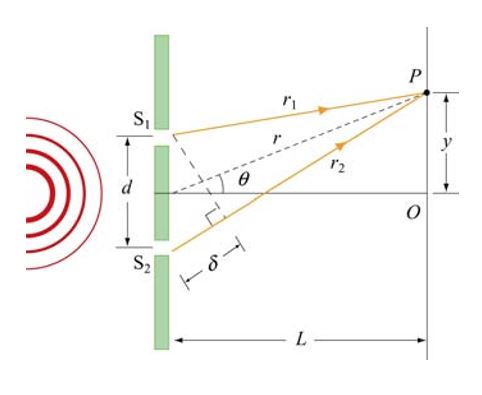
\includegraphics[scale=0.6]{notes/images/Interference-Single-Source-2.JPG}
    \caption{Double-slit experiment.}
\end{figure}
\FloatBarrier

Note that the problem is essentially identical to the two source interference experiment. To locate the positions of the fringes as measured vertically from the central point $O$, in addition to $L \gg d$, we shall also assume that the distance between the slits is much greater than the wavelength of the monochromatic light, $d \gg \lambda$. The conditions imply that the angle $\theta$ is very small, so we can apply the small angle approximations;
\begin{equation*}
    \sin \theta = \tan \theta = \frac{y}{L}
\end{equation*}

Substituting the above expression into the constructive and destructive interference conditions given in equations \ref{eq:path-difference-constructive} and \ref{eq:path-difference-destructive}, the positions of the bright and dark fringes are respectively,
\begin{equation}
    y_b = n \frac{\lambda L}{d}
\end{equation}
and
\begin{equation}
    y_d = \left(n - \frac{1}{2}\right) \frac{\lambda L}{d}.
\end{equation}
If we now consider the separation between two adjacent bright fringes $\Delta y$, we find that
\begin{equation*}
    \Delta y = \frac{\lambda L}{d},
\end{equation*}
which can be rearranged to solve for $\lambda$;
\begin{equation}
    \lambda = \frac{d \Delta y}{L}.
\end{equation}
Which is more commonly written as
\begin{equation}
    \lambda = \frac{ax}{D},
\end{equation}
where $x$ denotes the separation between two adjacent bright fringes (or two adjacent dark fringes), $a$ denotes the separation between the two slits and $D$ denotes the separation between the slits and the screen.